\documentclass{svproc}
\usepackage[font={small},skip=5pt]{caption}
\usepackage{graphicx} 
\usepackage{amsmath}
\usepackage[backend=biber,style=numeric,sorting=none]{biblatex}
\usepackage{tabularx}
\usepackage{algorithm}
\usepackage{algorithmic}
\usepackage{subfig}
\usepackage{booktabs}
\usepackage{float}
\usepackage{longtable}
\usepackage{hyperref}
\usepackage{wrapfig}
\usepackage[a4paper, margin=1in]{geometry}
\usepackage{url}
\usepackage{setspace}


\addbibresource{lit.bib}
\raggedbottom

\setlength{\abovecaptionskip}{5pt}  % Space above the caption
\setlength{\belowcaptionskip}{0pt}
\setstretch{0.95}
\setlength{\textfloatsep}{10pt} % Space between floats and text
\setlength{\floatsep}{8pt}      % Space between floats
\setlength{\intextsep}{8pt}     % Space between inline floats and text

\title{Time to Retrain? Evaluation of the CDSeer drift detection method in noisy and imbalanced minimal-supervision classification problems}
\author{Aleksandra Kaminska, Muhammad Zeeshan Babar}
\institute{University of Leeds, School of Computing, ODL MSc in AI, UK.}
\date{August 2025}

\begin{document}
\maketitle

\begin{abstract}
    Machine learning model pipelines in production have been shown to suffer from performance degradation over time due to data distribution and concept drift. Detecting the concept drift aspect can be particularly challenging in streaming, settings such as Internet of Things, especially when faced with scarcity of labelled points. \cite{pham2025} proposed a novel CDSeer concept detection method for such sparsely labelled problems. In this project we extend their evaluation of CDSeer to noisy and imbalanced problems and to wider set of drift type, as well as propose and evaluate adjustments to the CDSeer’s label querying strategy and pseudo-label propagation, demonstrating that while these amendments have their merits, they do not outperform the original CDSeer method in such information-poor problem settings.  
    
    \keywords{semi-supervised drift detection, concept drift detection, active online learning }
\end{abstract}

\section{Introduction}
    With machine learning models being increasingly deployed in a wide range of real-world contexts, the ongoing high, stable performance of these models becomes a crucial concern. At the same time, performance degradation of deployed models over time is a common occurrence, as data distributions and feature-label relationships evolve. Such degradation makes deployed models progressively less useful and reliable as the time since deployment increases. Periodic retraining and redeployment of models is a generally accepted remedy for these issues yet can be expensive – both computationally and due to the expert labelling required. Consequently, it is desirable to retrain models only when necessary, guided by reliable drift detection that reliably signals changes in model relevance.
    
    Detection of model drift has been an active area of research for a few decades, both in terms of detecting changes over time in input data distribution (“data drift”) and in terms of changing relationships between the input features and the model outputs (“concept drift”). Detecting data drift is often an easier problem and can be achieved using statistical techniques. Detection of concept drift is more challenging, and especially so in semi-supervised settings with low label availability (label scarcity), noise or class imbalance. These characteristics are common in Internet-of-Things (IoT) and similar high velocity streaming contexts, in which only a small fraction of instances can be labelled.
    
    \cite{pham2025} note that the leading concept drift detection methods in such high-volume, label-scarce settings often require excessive labelling and are typically not model-agnostic but rather optimised for specific model architectures. These are concerns to industry adoption, relaxing which would make deployment of model drift detectors in Machine Learning pipelines significantly more practical. 
    
    With that in mind, \cite{pham2025} propose a novel model-agnostic technique (“CDSeer”) for detecting concept drift in semi-supervised settings with high label scarcity and evaluate its performance on a selection of synthetic and real-world datasets. Their CDSeer method introduces a shadow model (“inspector”) that is trained in a semi-supervised manner on a recent subset of data and a small sample of recent expert-generated labels. The method relies on clustering of the recent data window to select a representative subset of points for which expert labels will be request. The most recently obtained labels are propagated to the recent data window via label propagation algorithm, and the results are used to train the shadow inspector model in a supervised manner. Difference in predictions between such shadow model are the reference model are then tracked by a standard supervised drift detector and used to detect concept drift change points.
    
    %\vspace{-10pt}
     \begin{wrapfigure}{r}{0.3\textwidth}
    	%\begin{figure}
    	\centering
    	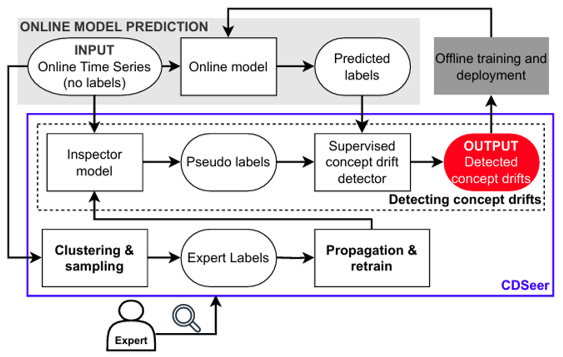
\includegraphics[scale=.40]{figures/Fig1_CDseer.png}
    	\caption{Overview of CDSeer method (\cite{pham2025}), p.4}
    	\label{fig:fig1}
    	%\end{figure}
    \end{wrapfigure}
    %\vspace{-10pt}
    
    In the CDSeer method, clustering and label propagation form a key part of the methodology, critical for the effectiveness of the drift detection. In their proposal \cite{pham2025} utilise Euclidean distance as a similarity metric for both clustering and for label propagation, without consideration of whether this type of metric is appropriate considering the type of relationship between features and target in a given problem domain. Indeed, this choice introduces implicit assumptions regarding the nature of the modelled concept, ones that might not necessarily hold in all the scenarios. It is possible that this assumption may lead to suboptimal clustering and suboptimal training of the shadow model in domains that exhibit more complex relationship between features and target. Furthermore, in evaluating and benchmarking the CDSeer performance, \cite{pham2025} have utilised a set of synthetic datasets which are all noise-free, balanced, exhibit exclusively abrupt concept drift and show no localisation of the drift, i.e. the concept drift generally occurs across entire population rather than for a select minority group. \cite{pham2025} also utilise a small number of real-world datasets in their assessment, however in absence of the ground truth about change points and types of concept drift, these datasets cannot compensate for the selectiveness of the synthetic datasets.
    
    
    In this project I aim to address these concerns by evaluating the CDSeer method on a wider selection of datasets, with particular focus on synthetic datasets with known drift points and exhibiting noise, class imbalance and varied types of concept drift including gradual and recurrent concept drift. I then propose several approaches to adjusting the CDSeer algorithm that could relax the constraints introduced via its clustering/label propagation approach and evaluate performance of these amendments against the original CDSeer algorithm.
    
    
\section{Literature Review}

Concept drift is a phenomenon in which the statistical properties of a target domain change over time in an arbitrary way (Lu, Zhang and Lu, 2014, p.1). Occurrence of concept drift has been identified as the root cause of decreasing performance in many real-world deployments of machine learning systems. Consequently, a need arises to be able to identify and adapt to such concept drift to avoid degradation in model reliability and reduced reliability of the model results.

%\vspace{-10pt}
\begin{wrapfigure}{r}{0.4\textwidth}
	%\begin{figure}
	\centering
	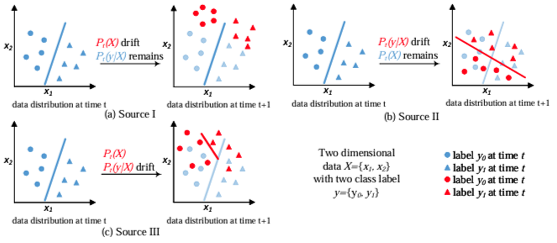
\includegraphics[scale=.6]{figures/Fig2_drift_sources.png}
	\caption{Sources of concept drift (Lu et al, 2018, p.3)}
	\label{fig:fig2}
	%\end{figure}
\end{wrapfigure}
%\vspace{-10pt}

Concept drift has been also referred to in literature as data drift, dataset shift, covariate shift and concept shift, often with slightly different meaning. Lu et al. (2018) systematise definition of concept drift as the problem in which $\exists{t}: P_t(X,y) \neq P_{t+1}(X,y)$ and subcategorise based on sources of the drift – source I caused by input data distribution only (“virtual drift”, “feature space drift”), source II caused exclusively by change in relationship between input features and target variables (“actual drift”, “decision boundary drift”), and source III representing a mixture of sources I and II. Following \cite{pham2025}, the focus for this project is drift owing to source II type, a.k.a. actual drift. Hereon within this report any references to concept drift should be taken to mean the actual drift, unless stated otherwise.

%\vspace{-10pt}
\begin{wrapfigure}{r}{0.3\textwidth}
	%\begin{figure}
	\centering
	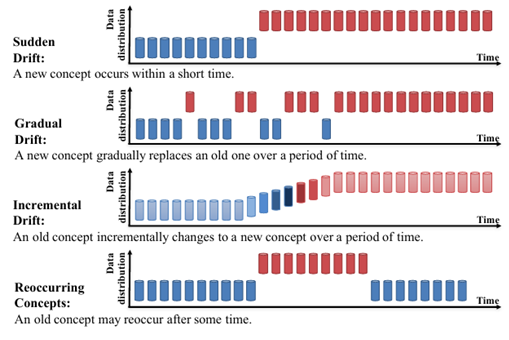
\includegraphics[scale=.5]{figures/Fig3_drift_types}
	\caption{Types of concept drift (Lu et al, 2018, p.3)}
	\label{fig:fig3}
	%\end{figure}
\end{wrapfigure}
%\vspace{-10pt}

Concept drift is commonly divided into four types – sudden drift, also referred to as abrupt drift; gradual drift; reoccurring drift, also referred to as recurrent drift; and incremental drift. The four types of concept drift are formally defined in \cite{gama2014} and \cite{lu2018} and illustrated in \ref{fig:fig3}. In their assessment of CDSeer method Pham et al. \cite{pham2025} have focussed solely on abrupt drift type datasets; this project aims to extend their assessment to other types of drift, with particular focus on gradual and recurrent drift.

Concept Drift Detection algorithms (CDDs) are categorised as supervised, semi-supervised and unsupervised based on their utilisation of ground truth labels. Unsupervised drift detectors do not utilise any ground truth labels and consequently can only detect drift if changes to input data distribution occur (virtual drift) and hence are not of interest in this report. Supervised drift detectors utilise true labels for all the data points, while semi-supervised methods utilise labels for some (usually few) data of the points. With the focus of \cite{pham2025} and this project on sparsely labelled, high volume streaming problems, the semi-supervised methods are of primary importance, while the supervised detectors serve as one of the building blocks for semi-supervised methods under consideration. 

Error Rate Based Detectors, which track changes to the error rate of base classifiers and raise a drift detection alarm when the change in the error rate is deemed to be statistically significant, form an important class of supervised and semi-supervised concept drift detectors. Gama et al. \cite{gama2014} classify error rate based drift detectors into three broad types: \textit{(1)} sequence-based methods, which evaluate prediction results sequentially in relation to a reference value (e.g. running mean) and report drift once a predetermined threshold/significance value is reached; such methods include CUSUM and Page-Hinkley (PH) \cite{sebastiao2017}, \textit{(2)} statistical-based methods, which calculate statistical parameters such as mean and standard deviation of predicted results, and report drift when these statics exhibit statistically significant shift; examples include DDM – classic drift detection method \cite{gama2004}, EDDM - an early drift detection method sensitive to gradual drift scenarios  \cite{baena2006}, ECDD – using exponentially weighted moving average detection \cite{ross2012}, or RDDM – reactive DDM \cite{barros2017}; and \textit{(3)} window-based methods, which utilise two different data instance windows for older and newer instances, and monitor divergence between the two windows; examples include ADWIN, HDDM – DDM based method utilising Hoeffding inequality \cite{frias2014}, or  Paired Learners  - a method using two different base learners, a stable one (focussed on entire set of data) and reactive one (focussed on recent data only), and monitoring changes in their relative predictions \cite{bach2008}. 

Paired Learners can be seen as an inspiration for the CDSeer drift detector defined in \cite{pham2025}, which also includes a classifier based on recent data as a gauge of drifting concept. Another recent important work on the topic is \cite{zhang2018}, utilising a long-term stable classifier and dynamic classifier to detect both sudden and gradual changes for online learning Concept Drift Detection.

Semi-supervised concept drift detection methods are more realistic than supervised ones in the streaming, big-data, high-velocity settings such as IoT environments, in which labels are not inherently available for new data points and need to be procured, subject to certain cost and effort. Semi-supervised CDDs require only a subset of data to be labelled, lessening the extent of the problem. Existing methods achieve that by selecting only most important data instances for labelling, utilising e.g. active learning – e.g. \cite{fan2004}, \cite{zhu2007}, and \cite{masud2010}; class imbalance \cite{lughofer2016}, classifier confidence \cite{haque2015}, \cite{haque2016}, grid density sampling \cite{sethi2016} or pseudo-error from classifier ensemble \cite{pinage2020}. However, these drift detection methods tend to be targeted towards reference models with specific ML architectures, as well as rely on very specific metrics to sample labels – both characteristics reduce their usability in general, model agnostic streaming settings.

Online active learning is a paradigm in machine learning that aims to select the most informative data points to label from a data stream and is particularly important topic in context of semi-supervised concept drift detection in general, and CDSeer algorithm \cite{pham2025} in particular. Cacciarelli and Kulahci \cite{cacciarelli2024} present a comprehensive survey of recent approaches to active learning for data streams, including the connection between active learning and semi-supervised learning for data streaming scenarios. As they point out, the widely analysed data problem of pool-based active learning \cite{aggarwal2014}; \cite{kumar2020} is not practical in most real-world streaming settings which are dynamic and of sequential nature. Instead in such scenarios one must perform online selective sampling \cite{hanneke2021}. Cacciarelli and Kulahci review the topic of budget constraints as applied to data annotation in this context, types and implications of latency in label availability, as well as different categories of strategies of instance selection criteria. Specifically, the diversity- and density-based approaches are the key category for the problem space outlined in \cite{pham2025}. These methods exploit the structural information of the input data space and aim to select data points representative of the overall distribution of data – including clustering used to label representative data points \cite{min2020}; \cite{ienco2014}, graph-based methods employed to explore the structure information of labelled and unlabelled data points \cite{zhang2020}, and methods building on the semi-supervised label propagation strategy \cite{long2008}.

Explainable AI (XAI) techniques have been explored in context of concept drift detection, both in context of detecting drift occurrences and in context of explaining the driving factors for these occurrences. Lunderberg and Lee prosed SHAP (Shapley additive explanations) method to measure the influence of each feature on model predictions \cite{lundberg2017}. Lundberg at al \cite{lundberg2020} further postulates that SHAP metrics allow to spot drift in features in predictive models. The topic of utilising XAI techniques has been an active research field, including \cite{haug2022}; \cite{lee2023}; \cite{tripathi2025}.


\section{Methodology}

The methodology and decisions utilised in this project fall within three categories: drift detector designs evaluated, datasets utilised, and finally the evaluation approach and metrics used. These are briefly outlined below, alongside the research questions that the project is looking to address.

\subsection{Research Questions}
This project focuses on the following questions.

\subsubsection{RQ1}\textit{Is CDSeer performance maintained on datasets with noise, class imbalance or complex decision boundaries?}

The synthetic datasets used to evaluate the CDSeer performance in drift detection in \cite{pham2025} are all class-balanced and without noise or redundant information. Furthermore, the datasets tend to have straightforward, typically linear decision boundaries. This project addresses this shortcoming by evaluating CDSeer method on a wider set of synthetic datasets exhibiting more realistic features such as noise and feature redundancy.

\subsubsection{RQ2}\textit{How does CDSeer perform in the presence of other drift types such as gradual or recurring drifts? Is the performance improved by utilising supervised drift detectors tailored towards such drift types?}

The synthetic datasets in \cite{pham2025} all exhibit abrupt, non-recurrent drift points only. This project examines how the CDSeer method performs on datasets exhibiting broader types of drift, in particular gradual drift and recurrent drift, and whether this performance is improved by using a tailored supervised drift detector such as EDDM \cite{baena2006} instead of general-purpose Page-Hinkley recommended in \cite{pham2025}.

\subsubsection{RQ3}\textit{At what threshold of expert label availability does CDSeer method become more effective in detecting drift than an outright supervised drift monitoring using only the (scarce) available expertly labelled subset of points? }

CDSeer method aims to detect drift by extrapolating pseudo-labels from the limited set of recent confirmed labels and train a shadow recency model using these pseudo-labels. Such an approach introduces assumptions about the structure of the data as well as certain approximation of results. The alternative would be to utilise a supervised drift detector with ground truth labels only, without resorting to extrapolation of pseudo labels. In this project I aim to explore the threshold of expert-label availability rate at which such a ground-truth only approach exhibits comparable performance to CDSeer, and how that threshold relates to the 0.6\%-0.8\% label availability rate assumed in \cite{pham2025}.

\subsubsection{RQ4}\textit{What effect do selected amendments to the clustering and label propagation approach, proposed by the author of this project, have on the overall effectiveness of CDSeer-like drift detector? }

CDSeer clustering and label propagation introduce implicit assumptions about the nature of the modelled problem and the relationship between features and target variable by utilising Euclidean-based similarity metric for both clustering and label propagation. That may not be appropriate for all use case sand may introduce unstable performance, leading to e.g. increased amount of false positive detections and unnecessary training cost. Similarly, the CDSeer method does not consider any preprocessing of data, such as scaling of points, in training the shadow model. While the shadow model is based on Random Forest and hence more resilient to unscaled data, the clustering and propagation itself may be affected by unscaled data, especially bearing in mind reliance on Euclidean distance metric, potentially leading to less effective drift detection. This project introduces a number of variations of the clustering/label propagation method in CDSeer and evaluates their performance against the original CDSeer method.


\subsection{Drift Detector Design}

\subsubsection{CDSeer Drift Detector}Pham et al. \cite{pham2025} have not made the implementation of the CDSeer drift detector public; hence the algorithm is reimplemented using the outline in \cite{pham2025}. Where the implementation details have not been provided by Pham et al. \cite{pham2025}, reasonable assumptions are made based on related literature and validated against the experiment results in \cite{pham2025}.

The CDSeer method is used for online drift detection and relies on tracking error rates between the reference model being monitored and the shadow model trained using a recent small sample of expert-provided labels (referred to in \cite{pham2025} as “inspector” model). For every new data point presented to the drift detector – from now on referred to as a step – a new shadow model is trained using a set of recent data points without labels (“inspector window”), and a very smaller set of recent expert-labelled data (“label memory”). The available ground truth labels are propagated to the rest of the inspector window using a label spreading algorithm, creating a set of pseud-labels. Furthermore, on every step the shadow model selects a subset of points from the inspector window that it considers representative and queries the oracle to obtain expert labels for all or some of the points, which are then used to update the label memory.

\begin{wrapfigure}{r}{0.4\textwidth}
	%\begin{figure}
	\centering
	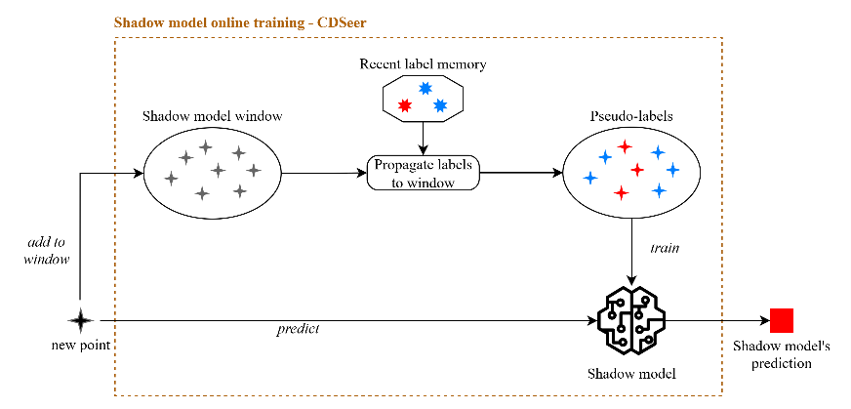
\includegraphics[scale=.6]{figures/Fig4_CDSeerSchema.png}
	\caption{Shadow model - online training step - original CDSeer}
	\label{fig:fig4}
	%\end{figure}
\end{wrapfigure}
%\vspace{-5pt}

In line with Pham et al. \cite{pham2025}, clustering, label spreading and training of the shadow model is performed on every step, except for the points used to train (or retrain) the reference model. Whether or not points used to retrain the reference model are also evaluated by the drift detector is dependent on the mode of evaluation being run (see Metrics and evaluation approach for details). The shadow model is an instance of a RandomForest model. The clustering uses DBSCAN method in the first instance, with epsilon parameter estimated using a simplified knee detection algorithm \cite{satopaa2011}. If the obtained clustering is not found to be sufficiently good, a KMeans clustering method is used instead. The label propagation is performed using Label Spreading algorithm \cite{bengio2004}. The RandomForest, DBSCAN, KMeans and LabelSpreading algorithms are implemented using scikit-learn library, with parameters as per Pham et al. \cite{pham2025}.

On the topic of procuring ground truth labels, Pham et al. \cite{pham2025} state only that stratified sampling is performed on the identified clusters, and that 15/10 (a hyperparameter) most recent labels are retained at any one time, without commenting on the specific sampling technique, the proportion of labels requested at each step, or whether immediate availability of labels is assumed. Consequently, in this project the expert label availability is controlled by two parameters – the proportion of inspector window that is requested for labelling in every step (“inspector curiosity ratio”) and the likelihood that the Oracle will provide a requested label (“compliance factor”), allowing to control for the expert label budget during the online drift detection steps. The stratified sampling utilises simple random sampling, while ensuring that at least one sample from each cluster is selected. It is assumed that there is no systematic delay in availability of labels, but rather they can be provided by Oracle synchronously. 

%\vspace{-10pt}
\begin{wrapfigure}{r}{0.4\textwidth}
	%\begin{figure}
	\centering
	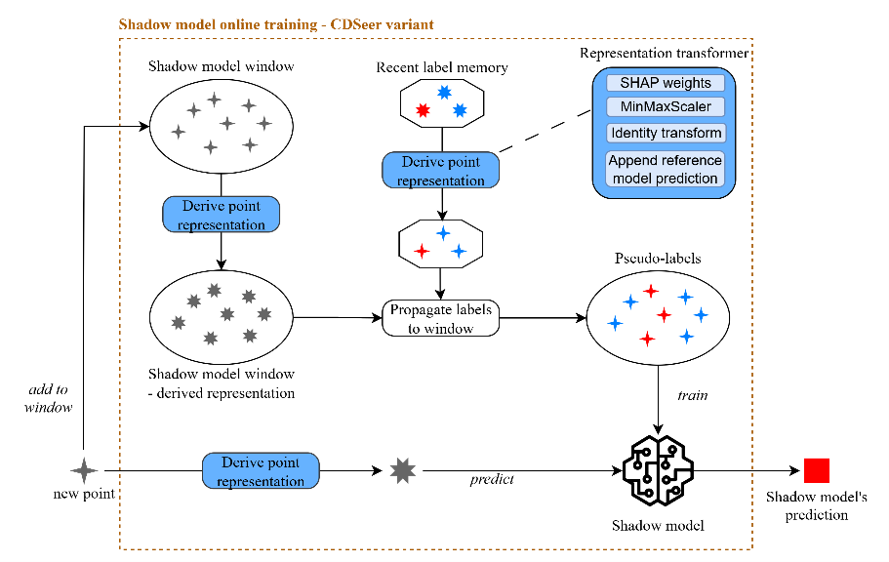
\includegraphics[scale=.6]{figures/Fig5_CDSeerVariantSchema.png}
	\caption{Shadow model - online training step - CDSeer variants}
	\label{fig:fig5}
	%\end{figure}
\end{wrapfigure}
%\vspace{-20pt}

Finally, CDSeer utilises a standard supervised drift detector for monitoring of the error rate. Pham et al. \cite{pham2025} name Page-Hinkley detector as the detector of choice, and for consistency the same detector is utilised in this project unless stated otherwise. It should however be noted that different detectors have been considered and experimented with as part of this project, most notably ADWIN, DDM, and FHDDM (Fast Hoeffding Drift Detection Method). Additionally, EDDM \cite{baena2006} has been used to evaluate \textbf{RQ3}. As an implementation note, the drift detectors’ implementations for the River machine learning library (\url{https://riverml.xyz/}) have been used in this project.




\subsubsection{Proposed CDSeer Adaptations}In this project several adaptations of the clustering/label-propagation approach in CDSeer are proposed, hypothesising that through different processing of the feature space, these variations may increase effectiveness and stability of the CDSeer-like drift detection in certain types of domains. These variations are evaluated against the original CDSeer algorithm.

\textbf{\textit{Clustering approaches}}
\begin{itemize}
	\item[Var1.]Scaling data prior to clustering and label propagation (“Scaling”). CDSeer’s usage of Euclidean distance in DBSCAN, KMeans and LabelSpreading means that differing ranges of different features in dataset may impact the derivation of pseudo-labels and affect stability of the drift detection algorithm. To counter this, the first CDSeer variant performs data scaling prior to clustering and propagation. The scale is based on the initial (offline) training set for the shadow inspector model, and transforms features to $[0,1]$ range using scikit-learn’s MinMaxScaler. Subsequently each point is transformed using this scaler as the first step of training the shadow inspector model.

\item[Var2.]Utilise SHAP values as coordinates of each point for clustering and label propagation (“SHAP”). In using Euclidean distance for clustering and label-spreading, CDSeer makes assumptions about shape of decision boundaries, roughly that neighbouring points typically have similar model outcomes. This assumption will not hold for some use cases, especially ones with complex decision boundaries. Var2 (“SHAP”) modification explores whether SHAP values of each data point might offer a better representation of the point for the purpose of clustering and pseudo-label derivation. The SHAP (SHapley Additive exPlanations) values are obtained using SHAP explainer, trained on the reference model and its training set. The SHAP explainer is implemented using KernelExplainer from SHAP package \url{https://shap.readthedocs.io/}.  

\item[Var3.]Combine coordinates of the point with output of reference model (“RefModel). Assuming the reference model being monitored is of sufficient quality, one could argue that nearby points (in terms of similarity metric used) should not be considered similar if they yield different outcomes of the reference model, as they do not form a cohesive cluster. In that spirit in Var3 adaptation the outcome of (up to date) reference model is considered when assessing points’ similarity for clustering and label propagation. Specifically, the model outcome is added as an additional dimension to the point representation. This does not as such eliminate the possibility of points with different outcomes ending up in same cluster, but it does allow the method to take the model outcomes into account when assessing similarity. Note that the same approach could be combine with SHAP representation in Var2.

\item[Var4.]Combine Scaling and RefModel – Var1 and Var2 (“Scaling + RefModel”). Scaling of data prior to clustering/propagation can be combined with supplementing the point representation with the outcomes of the (latest) reference model. 

\item[Var5.]Random selection of points for labelling. Pham et al. \cite{pham2025} on one hand define an involved procedure to cluster and recent points and select the candidates for labelling, while on the other hand do not seem to systematically consider the information gain aspects and work here and here on selecting best labels in active learning. One alternative then is to incorporate this this and this following on from reference and reference – this approach is not explored in this project. On the other end of spectrum one could select the points completely at random from the recent point window. Pham et al. \cite{pham2025} comment that this would be overly simplistic, without justification. In this project the random selection of points for labelling is benchmarked against the original CDSeer method to validate this assumption.

\item[Var6.]Supervised drift detection based on ground-truth expert labels only. The derivation of pseudo-labels in the CDSeer method allows to train the shadow model that can be used as a comparison to the reference model in the absence of ground-truth label values, in the hope that the recency of data used for shadow model will allow to spot the drift occurrence. However the derivation of pseudo-labels is necessarily based on certain assumptions and approximate, which may lead to substandard modelling and imprecise drift detection. Alternatively, one could ignore unlabelled points in drift detection and consider in a fully supervised manner only the points for which expert labels are available. Having said that the extreme scarcity of labels available in the setting outlined in CDSeer might mean there are simply not enough ground-truth labels available to spot any drift occurring. To quantify this, this project explores effectiveness of such supervised drift detection versus CDSeer method at different levels of label availability.

\end{itemize}

\textbf{\textit{Dimensionality Reduction}} The speed of processing is a key factor in the high-volume, high-velocity settings considered in this project – too slow processing of each point may result in being unable to make decision and detect drift in a timely manner. To enable the appropriate processing speed, this project performs dimensionality reduction through Singular Value Decomposition whenever a representation of a point exceeds a predefined number of dimensions. This is done so as to alleviate the computational burden.

\textbf{\textit{Label Propagation}} Any changes to the point representation described in variants 1-4 are also applied in label propagation, i.e. the same representation of each point is used both for clustering and for label propagation Variant 5 performs label propagation as outlined in the original CDSeer method, while variant 6 does not perform label propagation. 

\subsection{Datasets}

This project expands on the datasets used in \cite{pham2025} to evaluate CDSeer method, firstly by adding variations of these datasets that exhibit richer characteristics, and secondly by incorporating additional synthetic and real-life datasets. All the basic variants of the datasets below are widely used in concept drift detection research.

\subsubsection{Sine} A synthetic dataset with a decision boundary based on variations of sine function. Introduced by Gama et al. \cite{gama2004} The basic variant of this dataset used in \cite{pham2025} represents a binary classification problem, with features in the $[0,1]$ range, balanced and without noise. It exhibits two abrupt concept drifts, at 3,000 and 10,000 steps respectively, following the SINE1-REVERSE SINE1–SINE2 concept pattern. 

For this project, variations of the Sine dataset have been generated to add class imbalance, redundant features and scaling of feature subset. Furthermore, the concept order has been changed for some of the dataset variants, to follow the SINE2-REVERSE SINE2-SINE1 pattern to generate dataset with less simplistic decision boundaries – as SINE1’s and REVERSE SINE1’s boundaries approximate linear function.

\vspace{-10pt}
%\begin{wrapfigure}{r}{0.4\textwidth}
\begin{figure}
	\centering
	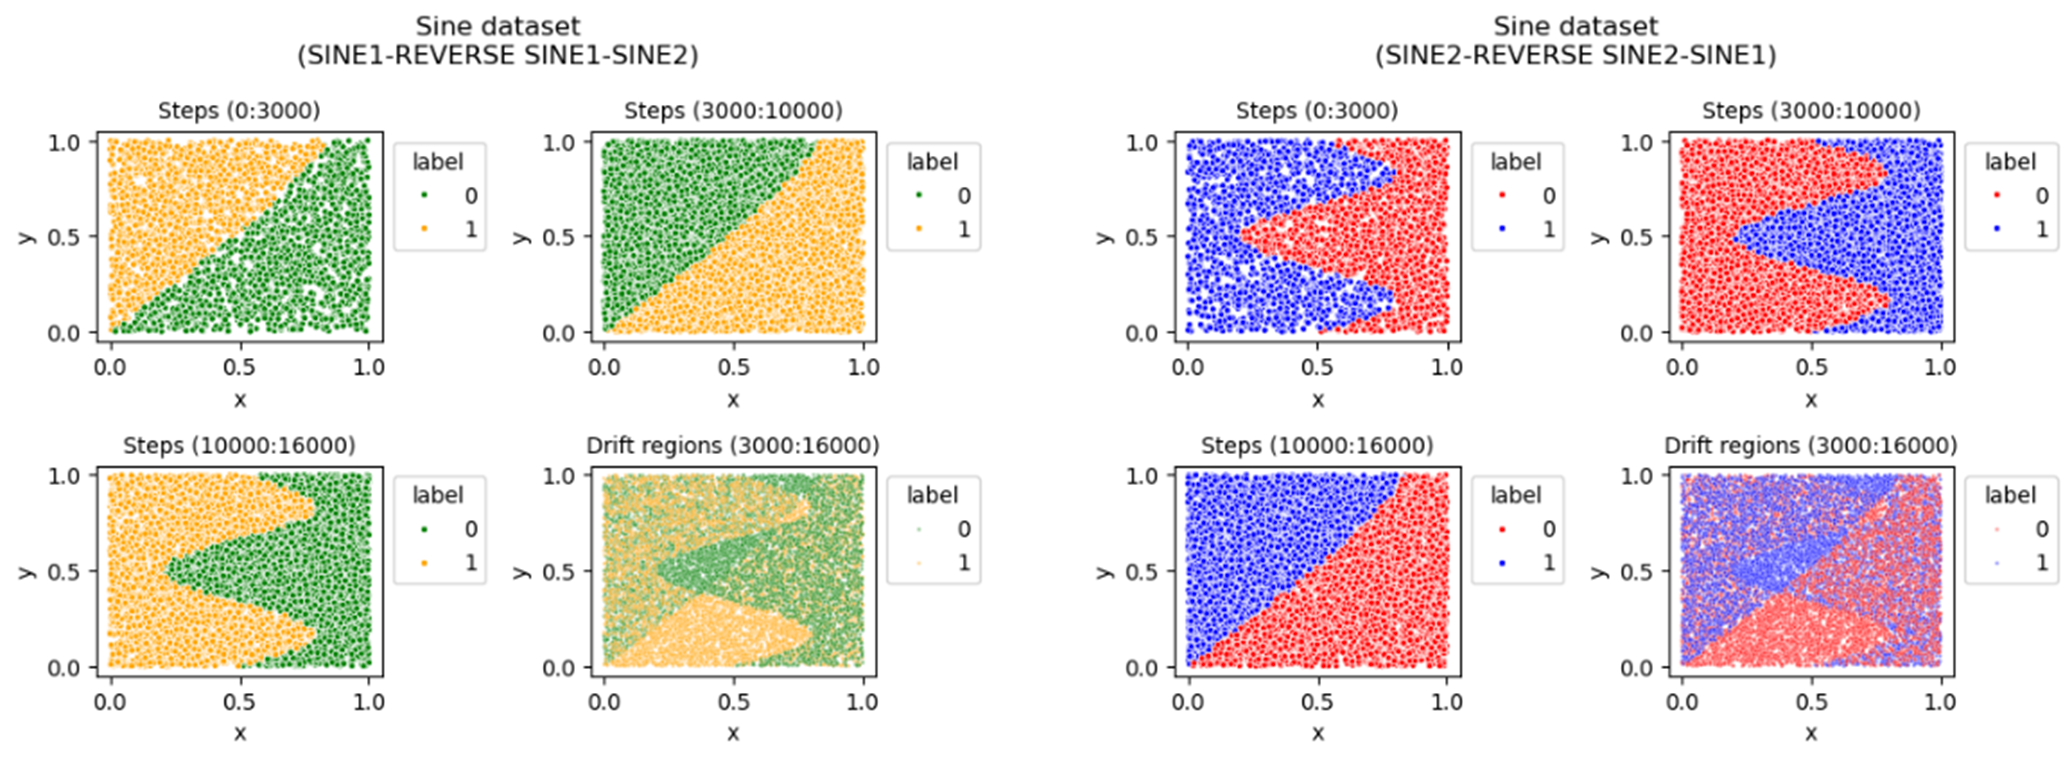
\includegraphics[scale=.6]{figures/Fig6_sine.png}
	\caption{Illustration of concepts and one of drift regions in Sine datasets}
	\label{fig:fig6}
\end{figure}
%\end{wrapfigure}
\vspace{-20pt}


\subsubsection{SEA}A synthetic dataset introduced by \cite{street2001}, with a decision boundary based on shifting linear function. The basic variant of this dataset used in \cite{pham2025} represents a binary classification problem, with features in the [0,10] range, balanced and without noise. It exhibits two abrupt concept drifts, at 3,000 and 10,000 steps respectively, following the Variant0-Variant1-Variant2 concept pattern. 

For this project, variations of the SEA dataset have been generated to add noise (at 2\% level), redundant features and scaling of feature subset. 


\subsubsection{Chocolate}Synthetic dataset, implementing lattice-like decision boundaries. Introduced by \cite{hu2024}, sourced from \url{https://github.com/THUFDD/THU-Concept-Drift-Datasets/tree/main}. Drift points are abrupt and occur after 20\%, 40\%, 60\% and 80\% of population. Drift exhibited by versions termed “abrupt” is also recurrent, whereas versions termed “sudden” have a smaller region of drift at each concept drift event due to the rotating nature of drift.  

For this project both a multi-label and binary versions of dataset have been generated, with and without noise and redundant features.

%\vspace{-10pt}
%\begin{wrapfigure}{r}{0.4\textwidth}
\begin{figure}
	\centering
	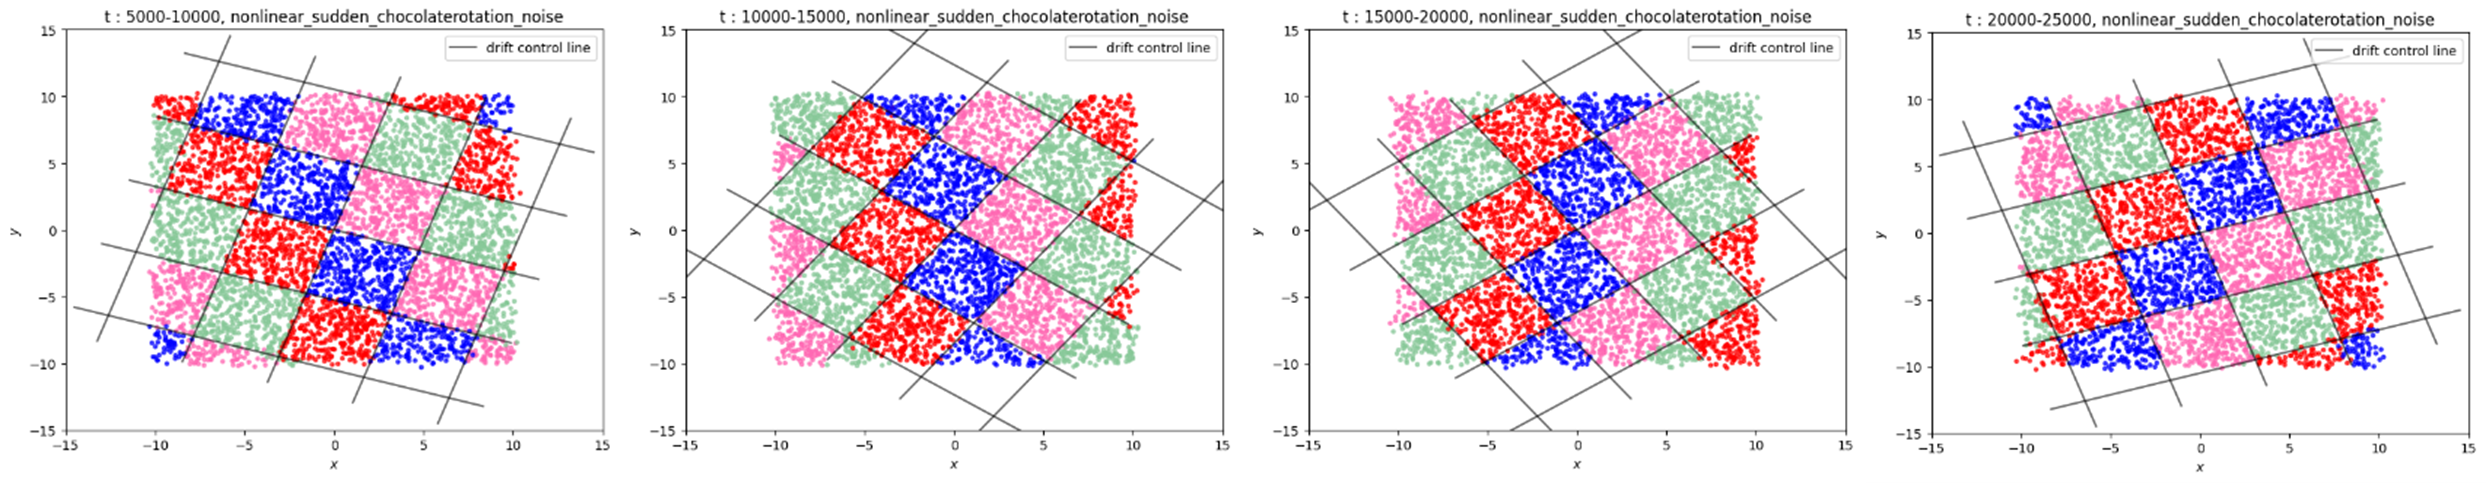
\includegraphics[scale=.6]{figures/Fig7_chocolate_multi.png}
	\caption{Multi-class rotating chocolate dataset after consecutive drifts}
	\label{fig:fig7}
\end{figure}
%\end{wrapfigure}


\vspace{-15pt}
%\begin{wrapfigure}{r}{0.4\textwidth}
\begin{figure}
	\centering
	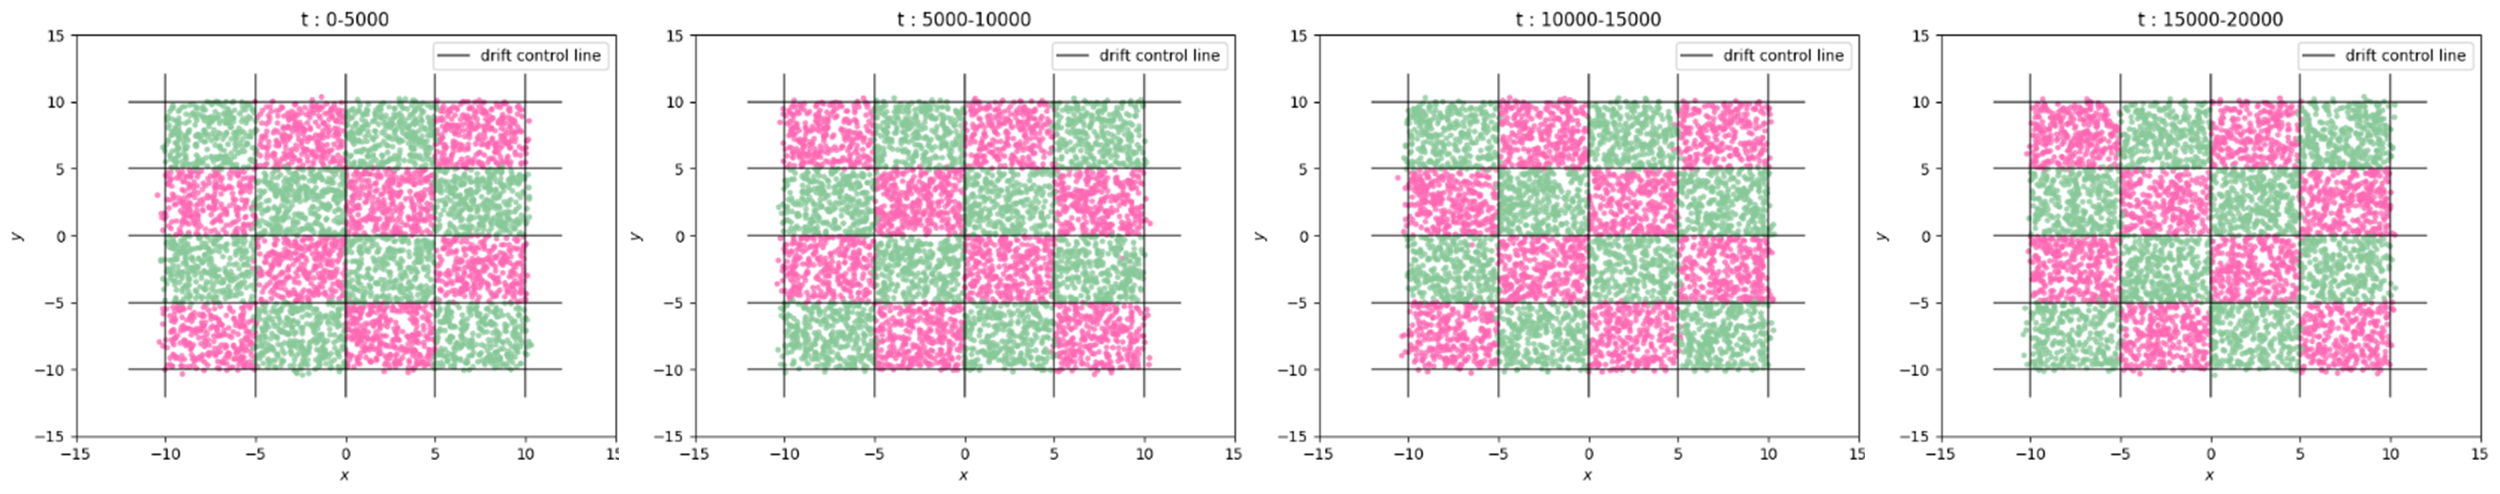
\includegraphics[scale=.6]{figures/Fig8_chocolate_binary.png}
	\caption{Binary non-rotating chocolate dataset after consecutive drifts}
	\label{fig:fig8}
\end{figure}
%\end{wrapfigure}
\vspace{-15pt}

\subsubsection{Harvard Concept Drift Datasets - Gradual Drift}A collection of synthetic datasets for concept drift detection testing, developed by \cite{lopez2020} and available from \url{https://dataverse.harvard.edu/dataset.xhtml?persistentId=doi:10.7910/DVN/5OWRGB}. 
The datasets all represent binary classification problems with 40,000 instances, 3 concept drift points and 4 concepts, with either abrupt or gradual drift. In this project only gradual drift versions are used, with drifts at time steps 9,500, 20,000 and 30,500, each with width of 1000. Detailed description of each dataset can be found in \cite{lopez2020}. Specifically, the following datasets are used in this project: 
\begin{itemize}
	\item sine\_0123\_gradual - 2 numerical features, a balanced binary class, and without noise. 
	\item sea\_3210\_gradual\_noise\_0.2, sea\_0123\_gradual\_noise\_0.2 - 3 numerical features (1 redundant), a balanced binary class, noise in concept with 0.2 probability.
	\item mixed\_1010\_gradual, mixed\_0101\_gradual - ruled by sequence of classification functions. 4 numerical features, a balanced binary class, and without noise.
	\item rt\_8873-9856-7896-2563, rt\_2563-7896-9856-8873 - ruled by a sequence of Random Tree functions. 2 numerical features, a balanced binary class, without noise.
\end{itemize}
It ought to be noted that the 20\% level of noise in the sea\_3210\_gradual\_noise\_0.2 and sea\_0123\_gradual\_noise\_0.2 goes beyond what would normally be considered a reasonable noise threshold and may affect the evaluation results due to challenges of reference model and/or shadow model in incorporating such a high noise threshold. Nonetheless the datasets have been used extensively in past works on drift detection, thus they have been included here for consistency.

\subsubsection{NOAA Weather Dataset (NOAA)}A subset of the original NOAA (National Oceanic and Atmospheric Administration) weather measurements dataset, containing 50 years of weather data from Offutt Air Force Base in Bellevue, Nebraska. The dataset prepared by \cite{ditzler2012} and sourced from \url{https://users.rowan.edu/~polikar/nse.html}.
This is a real-world dataset, frequently used in drift detection research. It represents an imbalanced binary classification task, with unknown drift points. Approximate drift points have been estimated using method outlined in \cite{pham2025}, for consistency with their evaluation of CDSeer.

\subsubsection{Electricity (Elec2)}Dataset representing electricity prices in New South Wales, Australia, introduced by \cite{harries1999}. The dataset covers a period of 2 years, with records taken every half an hour, and is a popular benchmark for testing concept drift detectors. 
It represents a binary classification problem (will the price go up or down), with real drift points unknown. Approximate drift points have been estimated using method outlined in \cite{pham2025}, for consistency with their evaluation of CDSeer. It ought to be noted that concerns have been raised by \cite{zliobaite2013} regarding the merit using this dataset for testing, however we have included it in this project for consistency with original benchmarking of CDSeer. 

\subsubsection{JiaoLong DSMS v2 (JIAOLONG)} A dataset collected by the National Deep Sea Center in Qingdao, Shandong, China, in the exploration task for the JiaoLong Deep-sea Manned Submersible on March 19, 2017. Introduced by \cite{liu2022} and sourced from \url{https://github.com/THUFDD/JiaolongDSMS_datasets}. 
\begin{wrapfigure}{r}{0.4\textwidth}
%\begin{figure}
	\centering
	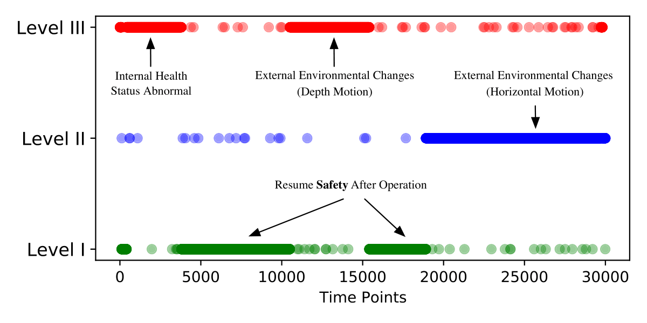
\includegraphics[scale=.6]{figures/Fig9_jiaolong.png}
	\caption{Indicative drift point ranges in JiaoLong DSMS dataset (from \cite{liu2022})}
	\label{fig:fig9}
%\end{figure}
\end{wrapfigure}
Data is the multi-variate time series with 24 features and 3 target classes, exhibiting slight class imbalance. The real concept drift points are unknown, but indicative regions have been described by \cite{liu2022} – see \ref{fig:fig9}. In this project the drift points have been estimated in line with methodology in \cite{pham2025}.

\subsubsection{Datasets Summary}Table in \ref{fig:fig10} summarises the key features of dataset families used in this project. More detailed description can be found in respective references within above description of each dataset, and in references.
%\begin{wrapfigure}{r}{0.4\textwidth}
\begin{figure}
	\centering
	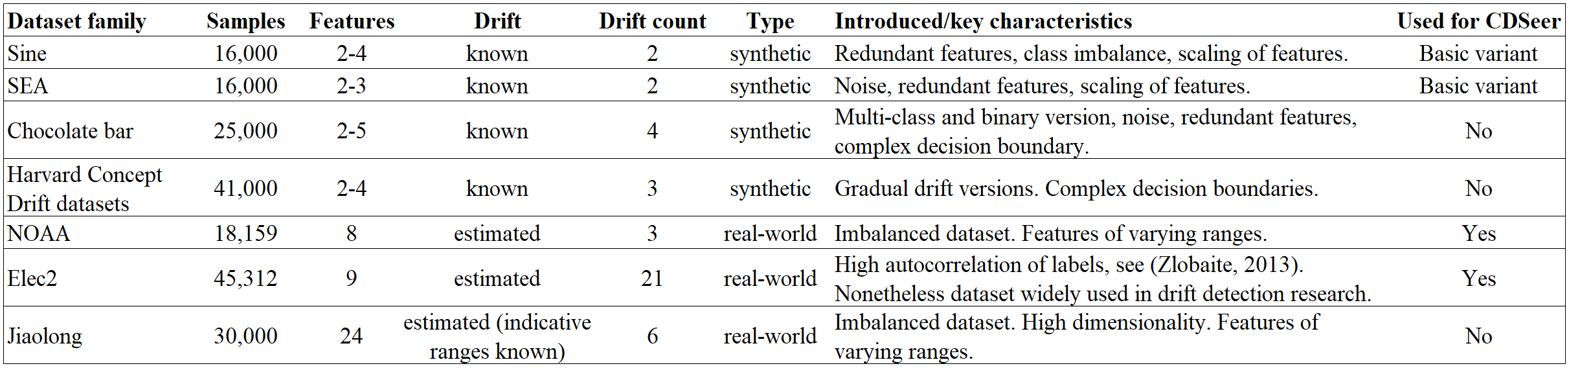
\includegraphics[scale=.7]{figures/Fig10_dataset_summary.png}
	\caption{Summary of datasets}
	\label{fig:fig10}
\end{figure}
%\end{wrapfigure}

\subsection{Evaluation Approach and Metrics}

\subsubsection{Metrics} Effectiveness of each version of drift detector is quantified using a set of measures related to the effectiveness of the drift detection, as well as to accuracy of the reference model retrained whenever the drift detection signals occur:
\begin{enumerate}
	\item \textbf{BalancedAccuracy and F1 of reference model predictions} Reference model is retrained when drift is detected, as described in Evaluation approach. section. The metrics are by comparing reference model predictions with ground truth labels and are calculated using all points on which reference model predictions have been obtained. For multi-label problems, the macro version of F1 metric is reported.
	\item \textbf{Drift precision and recall} Drift precision is the percentage of true positives of all the detected concept drifts by a CDD (Concept Drift Detector). Drift recall is the percentage of true positives detected by a CDD among all the GT concept drifts. 
\end{enumerate}

Drift detection is treated as correct of it occurs within $X$ steps (“tolerance”) after the ground truth drift. For non-gradual drift datasets with known drift points the $X$ values of 500, 1000 and 2000 are used, producing three different sets of measures. For datasets with gradual drift, a tolerance of 3000 is also used to approximately account for width of the drift. 

For datasets for which the drift points are not known, Pham et al. \cite{pham2025} estimate the ground truth drift points by using a supervised Page-Hinkley detector on the error rate generated by comparing predictions of reference model (without retraining) to the ground truth label. Such approximations are dependent on the specific reference model being tested, and affected by the quality of this model, and thus are highly approximate. Nonetheless the same approach has been used in this project for the sake of consistency with \cite{pham2025}.

For datasets with estimated drift, a 2-sided drift precision and recall metrics are calculated, in addition to metrics outlined above. 2-sided metric in this instance should be taken to mean a metric in which a detected drift is considered to be correct for the value of tolerance X, if such drift is \textit{either before or after} a ground truth drift, with the distance of at most X steps to that ground truth drift.

Furthermore, for selected experiments performance of the model at regular intervals is also examined, to illustrate the evolution of respective metrics, as well as the impact of general model suitability on quality of drift detection.

Finally, it should be noted that a measure corresponding to drift detection lag has been considered in place of fixed-width versions of drift precision and drift recall, as such measure is both relatively simple to understand and conveys a meaningful amount of information. However, this measure has been decided against to maintain consistency with \cite{pham2025} and their metric choices.

\subsubsection{Evaluation Approach} Each variant of the drift detection algorithm is evaluated using a variation of prequential evaluation approach, whereby following the initial training of reference model and of the shadow model, each subsequent point is presented to the reference model and to drift detection algorithm for assessment, and only it may be used to update the reference model – the (potential) updates of the model are described in more detail below. Furthermore, each set of evaluation results is obtained by averaging 5 consecutive evaluation runs, seeded with known seed values $(0, 1, …, 4)$.

The size of the dataset used for training the reference model ($WINDOW\_SIZE$), the number of most recent points visible (without labels) to the shadow model ($INSP\_SIZE$) and the size of shadow model’s memory for known recent labels ($MEM\_SIZE$) are all hyperparameters, as per \cite{pham2025}. Pham et al. \cite{pham2025} evaluate CDSeer for several combinations of these hyperparameters; for consistency with the most prominent of their results and unless indicated otherwise, this project utilizes $WINDOW\_SIZ$E of 1000, $INSP\_SIZE$ of 500, and $MEM\_SIZE$ of 15.

In prequential evaluation, the reference model would typically be updated with the new information (point) immediately after the point has been evaluated from prediction and drift detection perspective. However, the CDSeer detector is by definition meant to be model agnostic and thus one cannot assume that the reference model can be trained online. Consequently, in this project as in \cite{pham2025} it is assumed that model retraining occurs only once the drift has been detected.

Pham et al. \cite{pham2025} state that the retraining of the reference model is not within the scope of their paper, but that nonetheless as part of the evaluation they performed reference model retraining whenever drift has occurred. The details are not stated; however, the reproducing of their results suggests that the reference models have been retrained backwards, on the most recent points seen up to the moment of drift detection. This approach has the benefit of being able to immediately retrain the models without needing to wait for new points to come in (though one may need to await the derivation of labels for the points for training). It does however mean that the more efficient the drift detector is in terms of speed to detect drift, the more of pre-drift points will be used to train the new reference model. This is likely to lead to increase in false positive drift detections and makes the drift detectors appear less effective in evaluation. The alternative would be to train forward, using the first $WINDOW\_SIZE$ points following the drift. Such an approach would provide better reflection of effectiveness of the drift detector model by increasing the likelihood of each new version of reference model being trained on a coherent concept. It would however mean that not all the available points in the dataset could be used for evaluation of the drift detector.

Consistency with \cite{pham2025} demands that backwards retraining is used, however using the forward retraining approach would give more accurate view of effectiveness of drift detection methods being assessed. As a compromise both retraining methods are utilised in this project, with the specific method stated when discussing results. When comparisons are being made with \cite{pham2025} backward training is used, whereas in more general settings the forward training is preferred.

Lastly, the streaming nature of the problem is simulated by sequentially presenting each consecutive point to the reference model and drift detector algorithms, utilizing the  River framework – with the exception of points used for (re)training the reference model, which are processed offline in a batch manner.

\subsubsection{Implementation}

Implementation of this project is available on \url{https://github.com/kydrysek/CDSeer_Enhancements}, and access to the code can be requested. 
Below in algorithm \ref{algo1} we present as pseudocode the key aspects of modified drift detection in CDSeer variants.

\setlength{\textfloatsep}{5pt}
   \begin{algorithm}[H] 
	\begin{algorithmic}[1]
		\REQUIRE Trained reference model \( Model \), stream of input data \( Stream \) initialised supervised drift detector \( SDD \), shadow model \( Inspector \) and oracle \( Oracle \)
		\ENSURE Detection of concept drift, i.e. changes in relationship between model output and model inputs
		\STATE
		%\FOR{(point in stream)}
		\WHILE{( \( point \) in \( Stream \) \AND \NOT{ \( SDD \) detected drift)}}
		\STATE add \( point \) to  \( Oracle \)
		%\STATE \( model_prediction \leftarrow \text{Select}(s_0) \) \hfill \# \textbf{Selection}
		%\IF{ \( node \) is not a terminal node }
		\STATE \( modelPrediction \leftarrow \text{Model.predict}(point) \) 
		
		\hrulefill
		
		\textbf{Inspector prediction:}
				
		\STATE add \( point \) to  \( Inspector \) window \hfill \# \textbf{FIFO queue}
		\STATE \( pointRepresentation \leftarrow Inspector.transform(point) \) 
		\STATE
		\STATE derive \( clustering \) following CDSeer, using \(pointRepresentations\) for current \(window \) 
		\STATE \( pointsToRequest \leftarrow \text{StratifiedSample}(clustering) \) 
		
		\STATE request \(  labels(pointsToRequest) \) for \( Oracle \) \hfill \# \textbf{Asynchronous, labelling lag}				
		\STATE \( newLabels,labelledPoints \leftarrow Oracle.recentlyLabelled() \) \hfill \# \textbf{From this/previous requests}
		\STATE update short term memory of labels in \( Inspector \) using \( newLabels,labelledPoints \)
		\STATE		
		\STATE memoryRepresentations $\leftarrow$ \(\text{ transformed } labels \text{ from } memory\)
		\STATE \(pseudoLabels \leftarrow LabelSpreading(memoryRepresentations,memorylabels,windowRepresentations)\)
		\STATE \(Inspector \leftarrow Inspector.retrain(pseudoLabels,windowRepresentations) \) 
		\STATE
		\STATE \( inspPrediction \leftarrow \text{Inspector.predict}(point) \) \hfill \# \textbf{Always just trained} 
		
		\hrulefill
		\STATE update \(SDD\) detector with \textbf{prediction error value }\( (modelPred != inspPrediction) \)
		\STATE
		\ENDWHILE
		\STATE
		\STATE \textbf{return} signal for drift detection, so that model can be retrained and experiment reinitialised
	\end{algorithmic}
	\caption{Orchestration of drift detection using supervised detector and shadow model}
	\label{algo1}
\end{algorithm}

The critical differences in algorithm \ref{algo1} compared to original CDSeer method is consistent use for transformed representations for points, corresponding to derivation of SHAP coordinates, scaled coordinates or another suitable transformation,

These transformations are initialised when the Inspector shadow model is reinitialised, using information on points (not labels) corresponding to the training window for Inspector. These points are provided by the Oracle, and are used to e.g. train MinMaxScaler or SHAP Explainer.


\section{Experiment Results}

In performing the evaluation outlined above, several observations arise not only about the effectiveness of CDSeer and its variants, but also about the drift detection in general. Firstly, it is important to note that very fast and accurate detection of drift can worsen the performance of reference model, unless the appropriate steps are taken to shield the reference model from retraining on a significant amount of pre-drift data. This is demonstrated in \ref{fig:fig11} using one of the Chocolate datasets – a supervised drift detector with full label knowledge is so fast at spotting drift points that a model retrained on past data retrains mostly on pre-drift data, lowering its future performance. This does not present a problem if model is retrained on post-drift data (“forwards” version), but it does pose limitations on how quickly the new model can be available due to need to procure new labelled data.

\begin{wrapfigure}{r}{0.5\textwidth}
%\begin{figure}
	\centering
	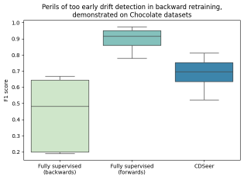
\includegraphics[scale=.5]{figures/Fig11_res.png}
	\caption{Accurate drift detection can, with substandard pipeline setup, lead to worse models}
	\label{fig:fig11}
%\end{figure}
\end{wrapfigure}
%\vspace{-20pt}

Furthermore, our experiments highlight another fundamental observation regarding reliance of drift detection performance on how well the reference model selected fits the target problem. If a particular model architecture is not particularly well suited to the task to hand and exhibits substandard performance even pre-drift, then a drift detector – CDSeer or otherwise – may well struggle to reliably detect drifting in the reference model as the model never predicted data accurately to start with. This also applies to the architecture used for shadow model, as in cases where it is not suitable to model the problem the inherent noise in the shadow model may obscure concept drifts. This is to an extent illustrated in the Harvard SEA dataset, owing to large proportion of noise in the dataset – see Appendix 2 \ref{sec:secApp2}. The good fit of the reference model for the use case is thus paramount, though realistically this is not a major concern as the performance would have been tested before deployment. Likewise, one also needs to consider for each problem the extent to which the RandomForest architecture with the sample size described in CDSeer is capable of effectively modelling the use case in question.

Additionally, we need to remember that while F1 (binary/macro) and Accuracy of the reference model with retraining are useful and relevant datapoints, they can be counterintuitive in that a poorly performing drift detector which generates a lot of false positive events would lead to frequent retraining of the model and hence artificially increased Accuracy / F1 of the reference model. This is illustrated for example in the performance of backwards-retrained CDSeer variants on the SEA dataset (see Appendix 2 \ref{sec:secApp2}). That performance would however come at the cost, both timewise and budgetary, of needing to retrain the model unnecessarily, and is something we explicitly want to avoid in our setting due to sparsely supervised nature of the data. 

Regarding \textbf{RQ1} and \textbf{RQ2}, in line with expectations, the CDSeer drift detection generally worsens in performance in presence of noisy datasets and of redundant variables – see Appendix 1 \ref{sec:secApp1}. It can also experience instability, in the sense of sometimes performing better and sometimes worse, for corresponding pairs of datasets e.g. with stretched input features (see the SEA datasets, stretched versions; Appendix 2 \ref{sec:secApp2}), or when faced with matching datasets with reversed order of concept (see Harvard dataset pairs, Appendix 2 \ref{sec:secApp2}). However, it needs to be noted that the supervised drift detection with full knowledge also drops in performance on these same datasets, as do the CDSeer variants introduced in this project – and crucially none of the proposed variants systematically remediates the drop in performance observed on such types of data in CDSeer. Nor is incorporation of EDDM strongly beneficial for gradual drift sets in our particular evaluations, The one exception to this is potentially performance of improvements on non-binary datasets. However, bearing in mind that majority of this datapoint is driven by performance of the MinMaxScaler amendment, this should nearly certainly be attributed to the specific characteristics of the multi-label dataset in this evaluation, namely the JiaoLong dataset and the Chocolate multi-label variants. Interestingly also, the querying of points at random for labels does not perform as badly as Pham et al. (2024) have assumed, and in a number of instances performs better than the original CDSeer – this minor effect can be observed across a number of different dataset characteristics. 

%\vspace{-10pt}
%\begin{wrapfigure}{r}{0.4\textwidth}
\begin{figure}
	\centering
	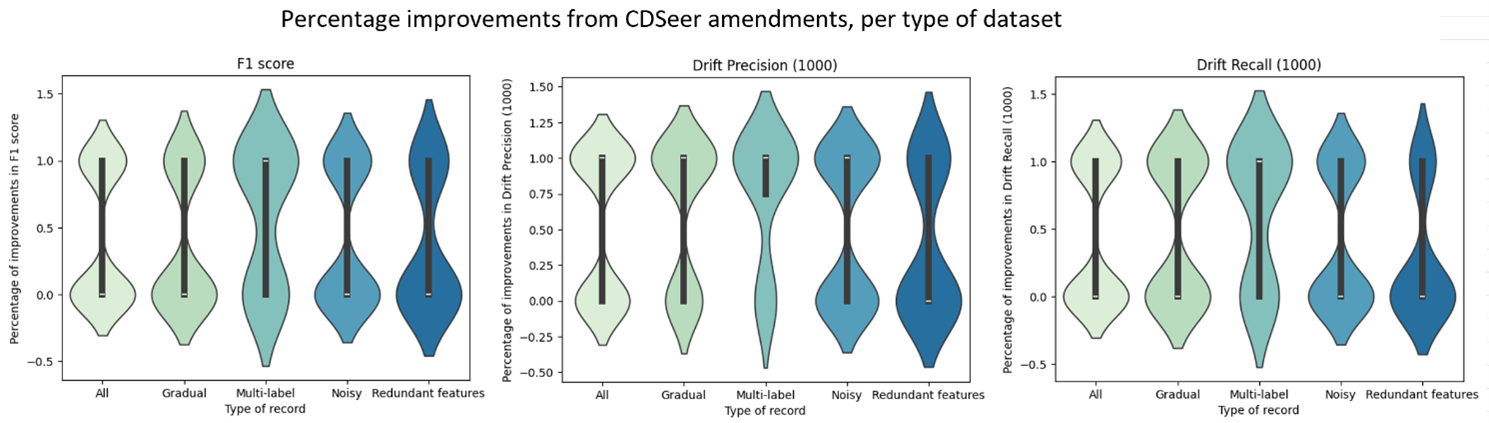
\includegraphics[scale=.7]{figures/Fig12_res.png}
	%\caption{Summary of datasets}
	\label{fig:fig12}
\end{figure}
%\end{wrapfigure}
%\vspace{-10pt}



On \textbf{RQ4}, none of the proposed improvements seem to systematically improve on performance of the original CDSeer. Some of them perform than others in particular situations, such as MinMaxScaler offering better stability and more consistent results for stretched versions of the same dataset, or models with more complex decision boundaries, like Chocolate datasets or Harvard Mixed and RT datasets, benefiting for appending of reference model predictions prior to clustering and label spreading – see SVC (Support Vector Classifier) results in Appendix 2 \ref{sec:secApp2}. Overall, however no single variant offers meaningful increase in drift detection performance for any of the types of datasets. Nonetheless the results show that all these adaptions have merit and possibly could be combined in a classifier ensemble – see section \ref{sec:secFutureWork} for further discussion.

\begin{wrapfigure}{r}{0.5\textwidth}
	%\begin{figure}
	\centering
	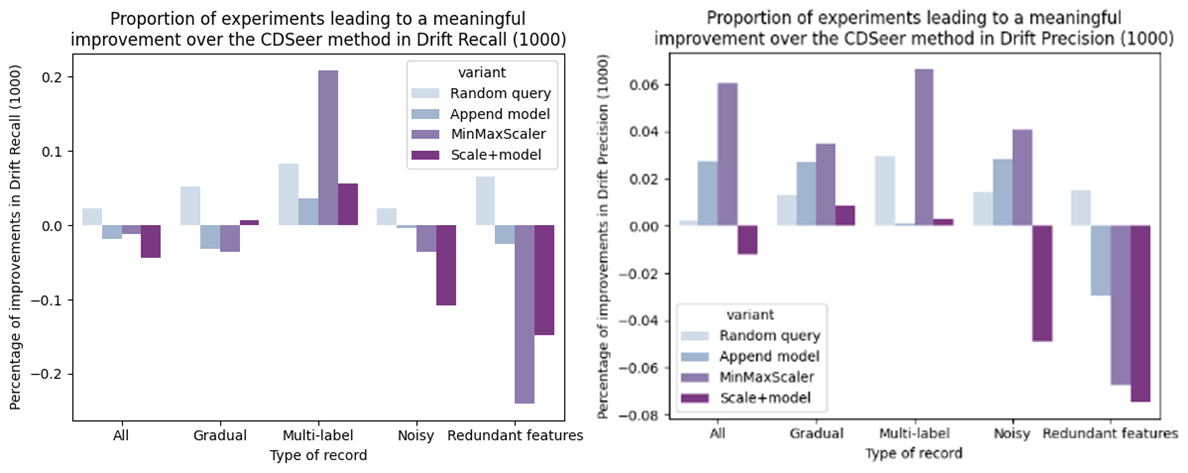
\includegraphics[scale=.7]{figures/Fig13_res.png}
	\caption{Random querying for labels as a valid procurement strategy}
	\label{fig:fig13}
	%\end{figure}
\end{wrapfigure}


It is worth noting that usage of SHAP weights does seem to hold promise, as in a5 number of runs across three different families of datasets (Harvard,SEA and SINE), the drift recall, accuracy and F1 all showed signs of improving for a significant number of datasets. Specifically the SHAP-only coordinates  fared better in over 50\% of runs, and were also close to 50\% of instances improved in case of drift precision. The version that combines SHAP coordinates with reference model output fared a bit worse, particularly in terms of precision. It did however still provide a level of improvement that ought to be further analysed.

\begin{table}[h!]
	\centering
	\resizebox{1\textwidth}{!}{%
		\begin{tabular}{|l|c|c|c|c|c|c|}
			\hline
			\textbf{Variant} & \textbf{Total runs} & \textbf{F1} & \textbf{Drift precision (1000)} & \textbf{Drift recall (1000)} & \textbf{Drift precision (2000)} & \textbf{Drift recall (2000)} \\
			\hline
			Both SHAP     & 44 & 63.636\% & 40.909\% & 65.909\% & 38.636\% & 59.091\% \\
			SHAP only     & 26 & 65.385\% & 46.154\% & 38.462\% & 50.000\% & 50.000\% \\
			SHAP+model    & 18 & 50.000\% & 16.667\% & 61.111\% & 11.111\% & 27.778\% \\
			\hline
		\end{tabular}
	}
	\caption{Performance metrics across different SHAP variants}
\end{table}




Lastly on the \textbf{RQ3}, CDSeer does appear to be meaningfully more effective than a method which does not attempt to produce pseudo-labels but rather perform supervised drift detection with only the sparse labels available. That is true even at meaningful amounts of label availability, such as 10\% availability. This makes sense instinctively, as derivation of sparse data points lead to slow and very inefficient drift detection; while at the same time the pseudo-labels generated by CDSeer method encode mostly realistic assumptions about similarity of samples and their outcomes, creating a sufficiently good proxy dataset on which to apply frequent drift detection.
    
    
    

\section{Conclusion and Future Work}
\label{sec:secFutureWork}

We have filled in the gap in \cite{pham2025} by performing a more comprehensive evaluation of CDSeer detector's performance on datasets with challenging characteristics, such as noise, imbalance or gradual drift. Further, we have proposed several amendments to the architecture of the shadow model in CDSeer method and evaluated performance of these amendments against the performance of original CDseer method. We have ascertained that the CDSeer method \cite{pham2025}  does actually perform much more reliably than originally expected even in noisy or imbalanced environments, and to an extent in presence of gradual drift, despite its assumptions regarding suitability of Euclidean distance similarity for comparing model outcomes. This conclusion makes sense in the context of the very scarce availability of the labels in the problem outlined – in the region of 0.6\%-0.8\%. With such extreme label scarcity, the label querying method introduced in CDSeer is just as good as most others, though as we’ve observed random querying would also be a suitable alternative – in a nutshell, in the problem setting there is so little information available that the set of assumptions introduced through the clustering and pseudo-label derivation in CDSeer are not any more detrimental than assumptions of any other label querying strategy with similar level of information utilisation. Having said, there are other avenues that we think are worth following, in particular in context of multiple hypothesis test drift detection  and further adaptions for gradual concept drift – see below. 

As we have observed in this project, different label querying strategies lend are most suitable to different use cases and datasets. Thus, us a follow up it would be worth exploring how best multiple hypothesis test drift detection \cite{lu2018} can be utilised in sparsely supervised concept drift detection methods such as CDSeer, particularly focusing on the parallel multiple hypothesis tests. Furthermore, in defining CDSeer Pham et al. \cite{pham2025} state that shadow model is implemented by a random forest. In future work it would be worthwhile to explore other models as a base for the shadow model: \textit{(1)} similarity based model such as KNearestNeighbours, acknowledging the similarity assumptions already implicit in CDSeer label querying and propagation, and \textit{(2)} online models, such as Mondrian Forests \cite{lakshminarayanan2014} or Adaptive Random Forests \cite{gomes2017}, to avoid the need to train shadow model from scratch for every prediction.

To further the work on suitability of CDSeer for gradual drift, we propose to evaluate wider range of detectors targeted towards gradual drift, such as FW-DDM \cite{liu2017}, ECDD \cite{ross2012}, or ensemble of classifiers methods \cite{zhu2007}. In addition to gradual drift suitability enhancements, one also ought to investigate performance of CDSeer and variants on problems with drift restricted to a minority subset, a problem that has been shown by \cite{giobergia2024} to be a challenge for many drift detectors. Furthermore, future work should perform a more comprehensive analysis and approach to label budgeting, in particular accounting for lag in expert label availability and assessing impact that has on efficiency of label propagation and shadow model training.

Finally, it would be interesting to look at applying Explainable AI techniques to try to achieve causal explainability of detected drifts, which could lead to actionable insights, following on from ideas presented by \cite{komnick2025}. 


\printbibliography
 
 \section{Appendix 1: Further Illustration of Results}
 \label{sec:secApp1}
 This appendix contains further comparisons of the CDSeer variants introduced in this project and their relative performance on different types of datasets. Figure \ref{fig:fig14} presents the results at the overall level of types of datasets characteristics, while figure \ref{fig:fig15} breaks down results by the specific CDSeer amendment considered.
 
 %\begin{wrapfigure}{r}{0.5\textwidth}
 \begin{figure}
 	\centering
 	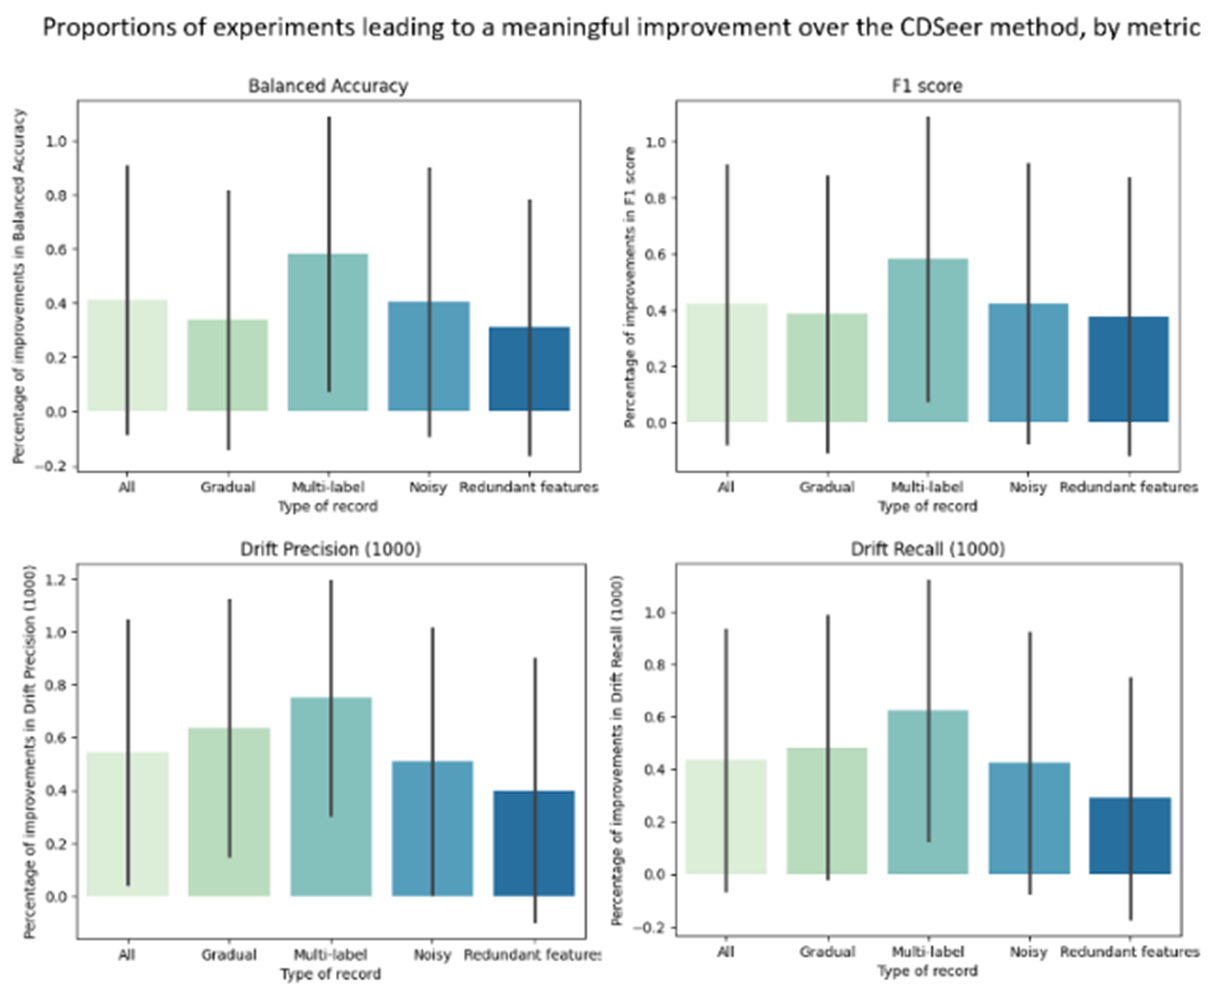
\includegraphics[scale=.7]{figures/Fig14_composite.png}
 	\caption{Types of datasets benefitting from one of the proposed amendments (non-SHAP)}
 	\label{fig:fig14}
\end{figure}
 %\end{wrapfigure}
 
  %\begin{wrapfigure}{r}{0.5\textwidth}
 \begin{figure}
 	\centering
 	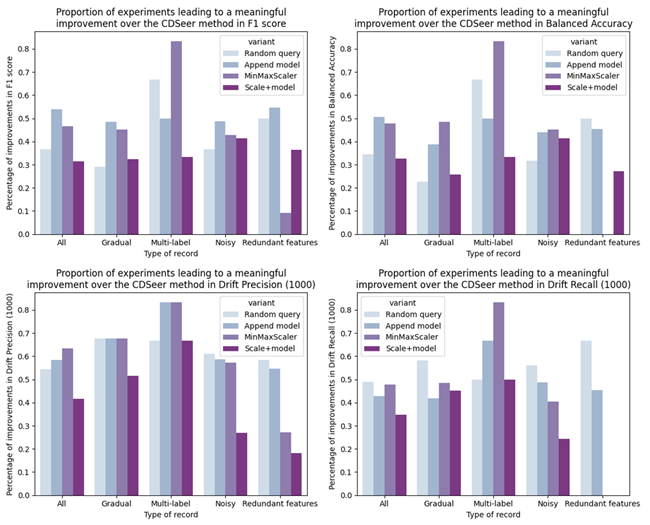
\includegraphics[scale=.7]{figures/Fig15_composite.png}
 	\caption{Proportion of experiments showing minor benefits from adjusting querying strategy (non-SHAP)}
 	\label{fig:fig15}
 \end{figure}
 %\end{wrapfigure}
 
   %\begin{wrapfigure}{r}{0.5\textwidth}
 	\begin{figure}
 	\centering
 	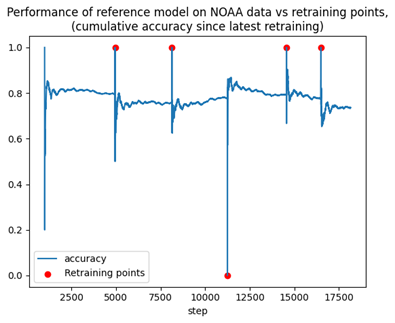
\includegraphics[scale=.7]{figures/Fig16_model.png}
 	\caption{Sample performance of reference model with retraining, measured by accuracy since last retraining}
 	\label{fig:fig16}
 	\end{figure}
 %\end{wrapfigure}
 
 Further figure \ref{fig:fig16} illustrates performance of a sample reference model with retraining due to drift detection – the spikes in accuracy are due to retraining of the model and restart of accuracy calculation (for the purposes of this illustration).
 

 
 \begin{figure}
 	%\centering 	
 	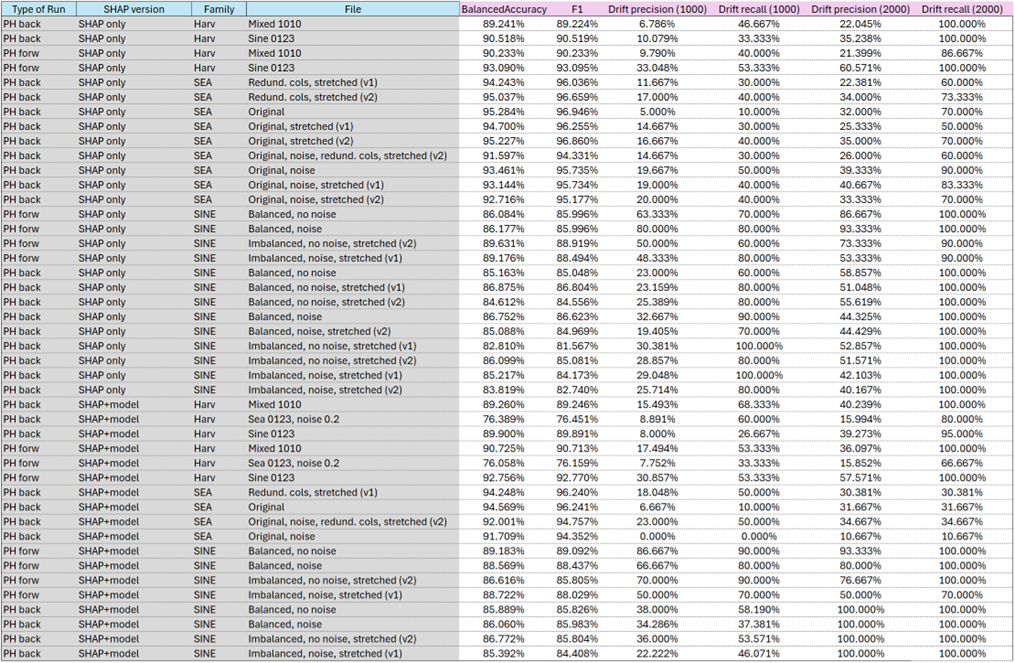
\includegraphics[scale=.95]{figures/Fig17_SHAP results.png}
 	\caption{Sample performance of reference model with retraining, measured by accuracy since last retraining}
 	\label{fig:fig17}
 \end{figure}
  
 
 Finally figure \ref{fig:fig17} presents a breakdown of performance of SHAP-variant runs benchmarked to the corresponding CDSeer results.
 
 
 
 
 \section{Appendix 2: Results by Dataset Family}
 \label{sec:secApp2}
 This appendix showcases selected results of evaluations performed. It is organised by the family of the dataset, and in one instance by type of reference model. In most cases both results for “backwards” retraining and the “forwards” mode are presented.
 
 Note that results highlighted in bright green background represent metrics where a proposed CDSeer variant improves upon the original proposed in \cite{pham2025}. Results highlighted with light blue background represent metrics of the same value as those for corresponding (original) CDSeer method.
 
 \subsection{Real-World Datasets - NOAA, JIAOLONG, ELEC}
  \begin{figure}
 	%\centering
 	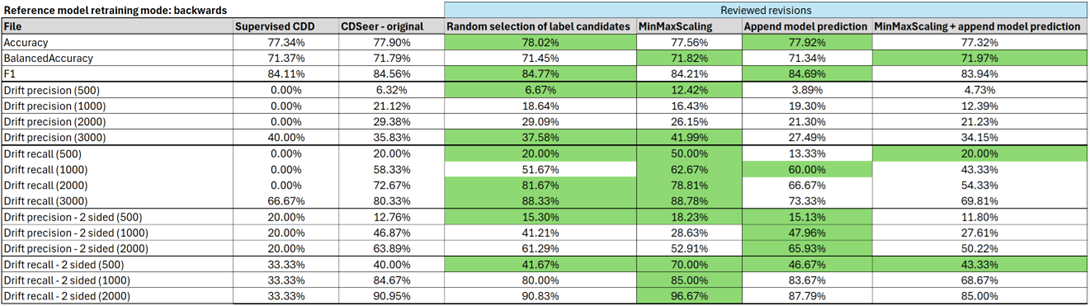
\includegraphics[scale=.95]{figures/Fig18_NOAA_1.png}
 	\caption{Results for NOAA dataset across all variants, in backwards retraining mode}
 	\label{fig:fig18}
 \end{figure}
 
 
 \begin{figure}
 	\centering
 	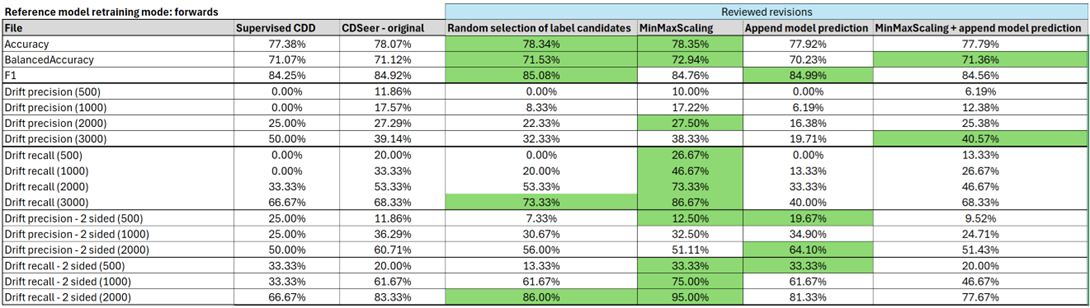
\includegraphics[scale=.95]{figures/Fig19_NOAA_2.png}
 	\caption{Results for NOAA dataset across all variants, in forwards retraining mode}
 	\label{fig:fig19}
\end{figure}
 
 %\subsection{JIAOLONG}
 
   \begin{figure}
 	\centering
 	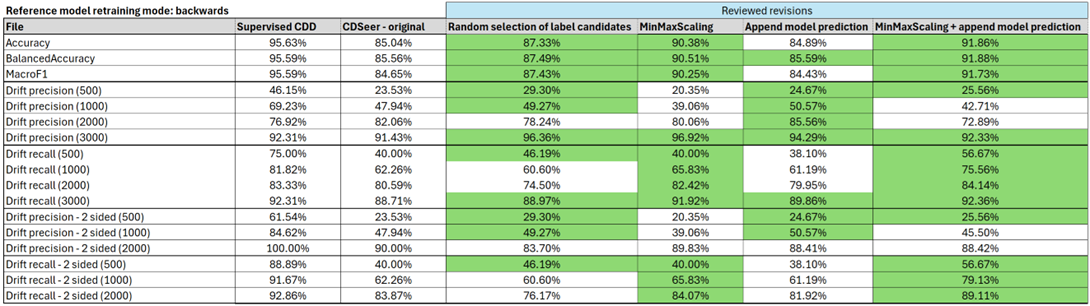
\includegraphics[scale=.95]{figures/Fig20_JIAOLONG_1.png}
 	\caption{Results for JiaoLong dataset across all variants, in backwards retraining mode}
 	\label{fig:fig20}
 \end{figure}
 
 
 \begin{figure}
 	\centering
 	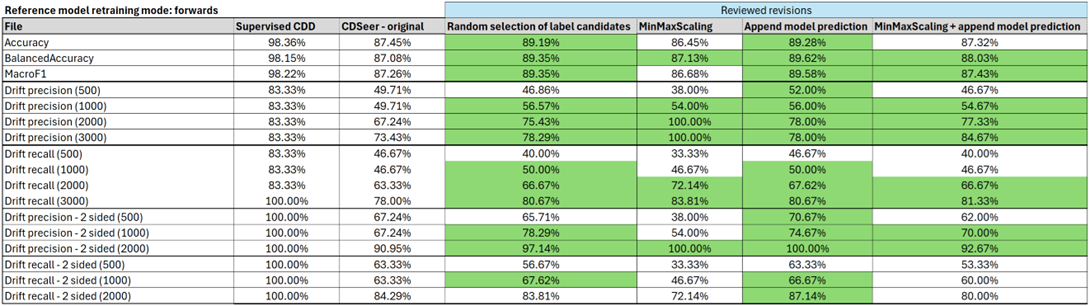
\includegraphics[scale=.95]{figures/Fig21_JIAOLONG_2.png}
 	\caption{Results for JiaoLong dataset across all variants, in forwards retraining mode}
 	\label{fig:fig21}
 \end{figure}
 
 %\subsection{ELEC}
 
 \begin{figure}
 	\centering
 	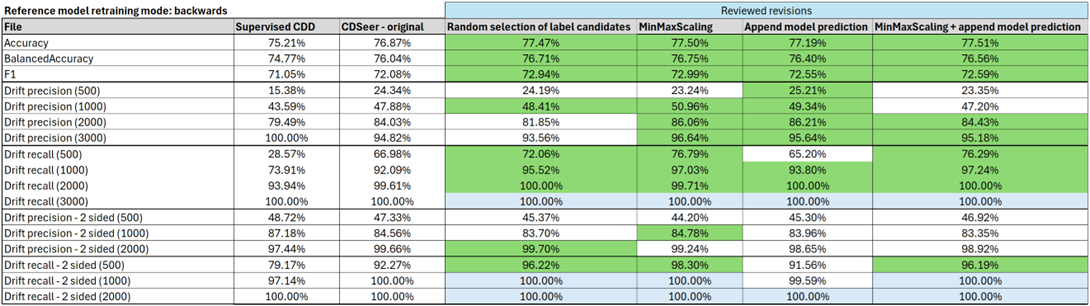
\includegraphics[scale=.95]{figures/Fig22_ELEC_1.png}
 	\caption{Results for ELEC dataset across all variants, in backwards retraining mode}
 	\label{fig:fig22}
 \end{figure}
 
 
 \begin{figure}
 	\centering
 	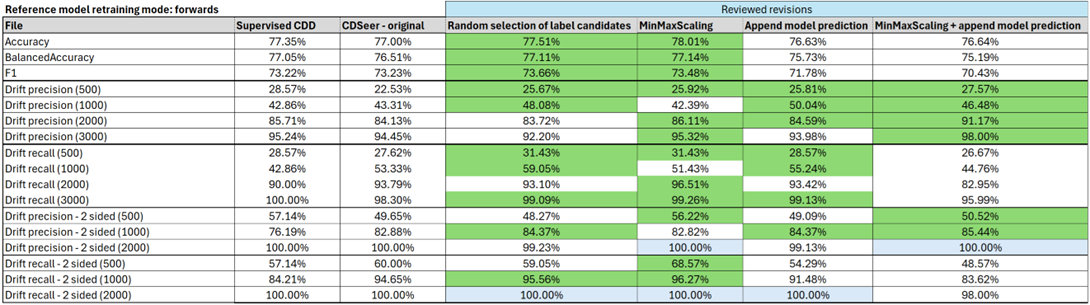
\includegraphics[scale=.95]{figures/Fig23_ELEC_2.png}
 	\caption{Results for ELEC dataset across all variants, in forwards retraining mode}
 	\label{fig:fig23}
 \end{figure}
 
 
 \subsection{Synthetic Datasets}
 \begin{figure}
 	\centering
 	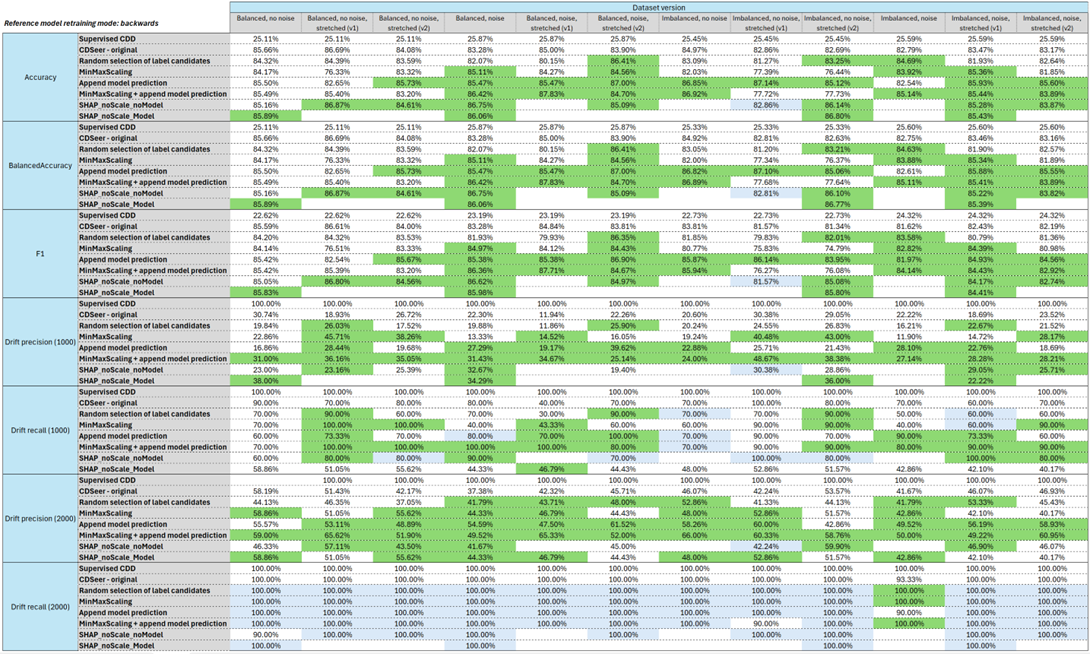
\includegraphics[scale=.95]{figures/Fig24_SINE_1.png}
 	\caption{Results for SINE datasets across all variants, in backwards retraining mode}
 	\label{fig:fig24}
 \end{figure}
 
 
 \begin{figure}
 	\centering
 	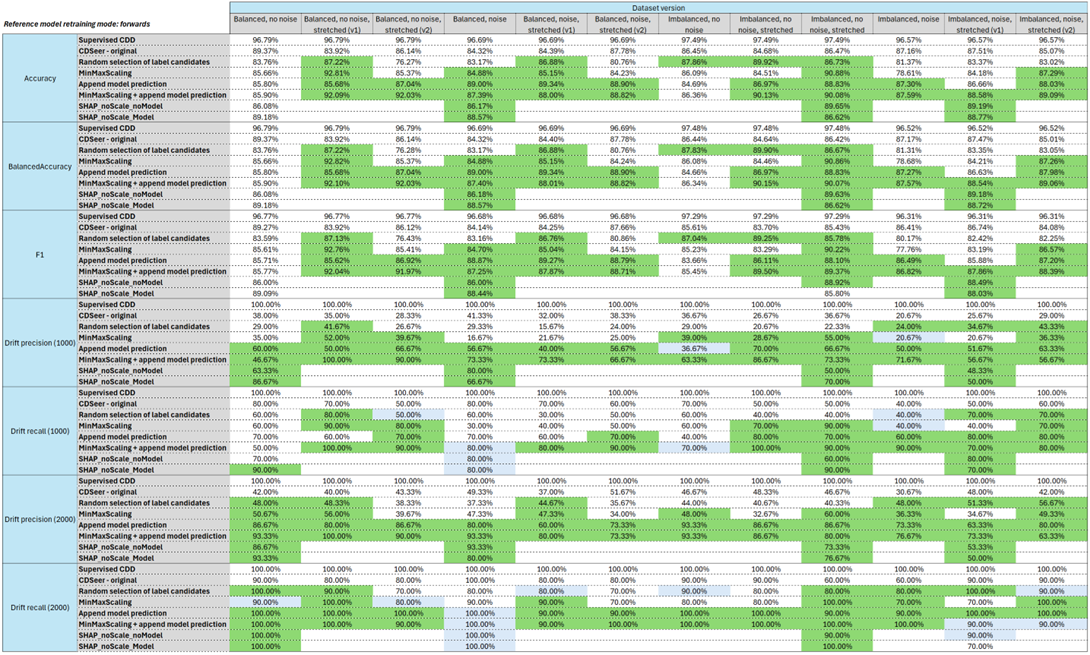
\includegraphics[scale=.95]{figures/Fig25_SINE_2.png}
 	\caption{Results for SINE datasets across all variants, in forwards retraining mode}
 	\label{fig:fig25}
 \end{figure}
 
 %\subsection{SEA}
 
 \begin{figure}
 	\centering
 	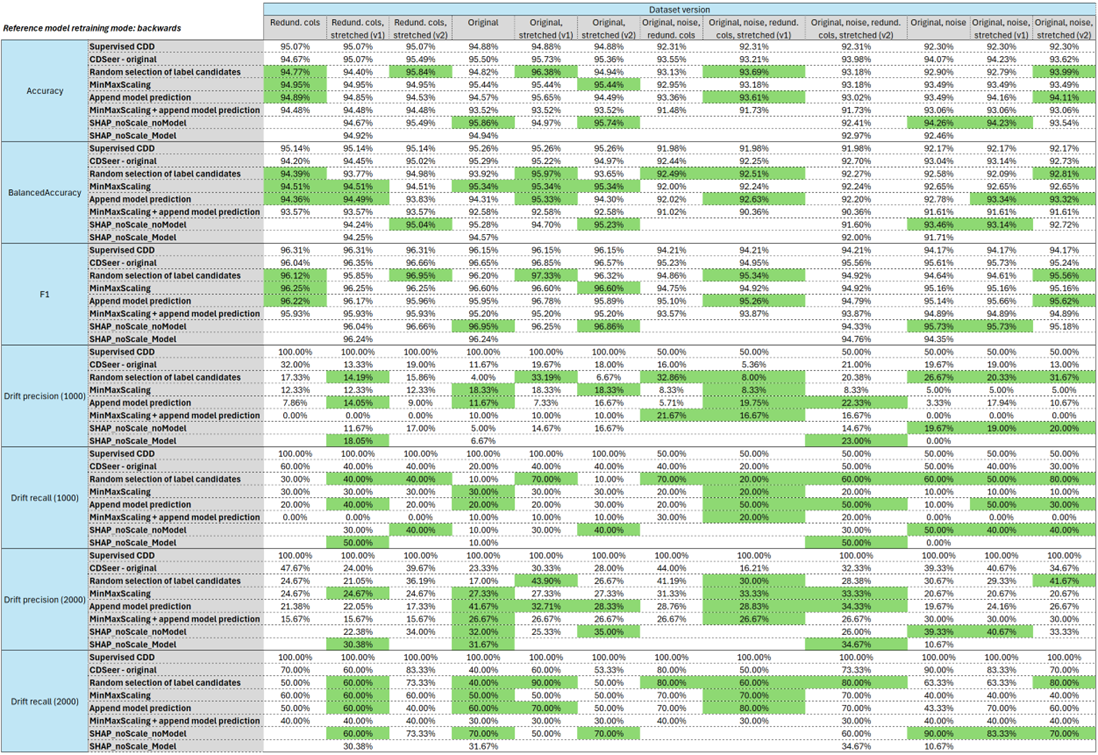
\includegraphics[scale=.95]{figures/Fig26_SEA_1.png}
 	\caption{Results for SEA datasets across all variants, in backwards retraining mode}
 	\label{fig:fig26}
 \end{figure}
 
 %\subsection{SVC}
 \begin{figure}
 	\centering
 	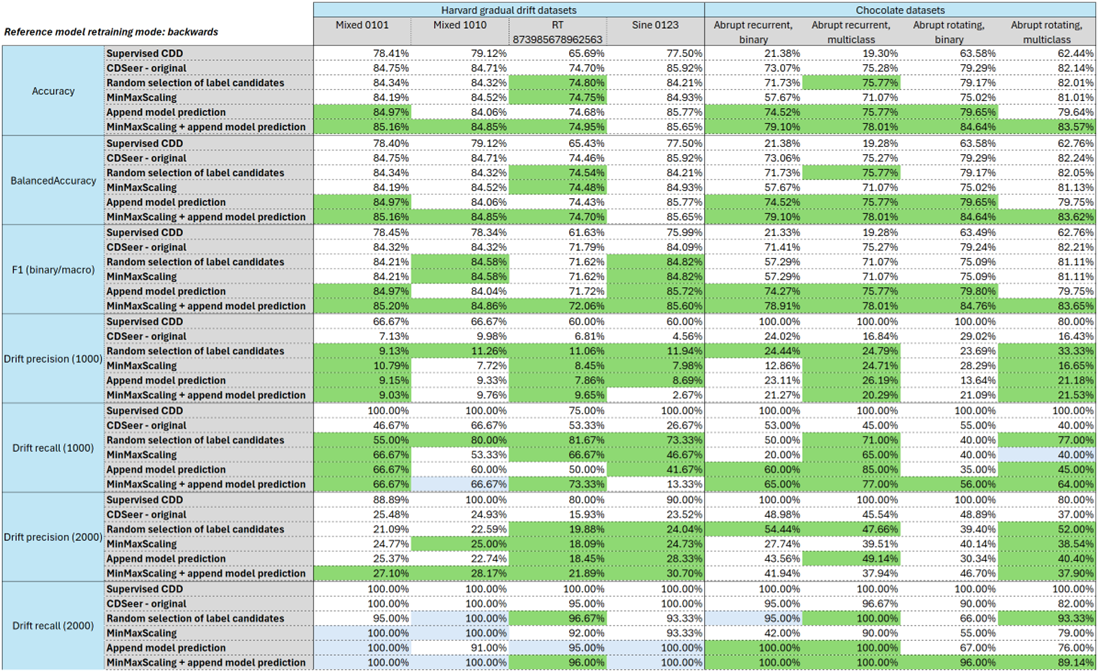
\includegraphics[scale=.95]{figures/Fig27_SVC_1.png}
 	\caption{Results for Harvard and Chocolate datasets with SVC reference model, in backwards retraining mode}
 	\label{fig:fig27}
 \end{figure}
 
 
 \begin{figure}
 	\centering
 	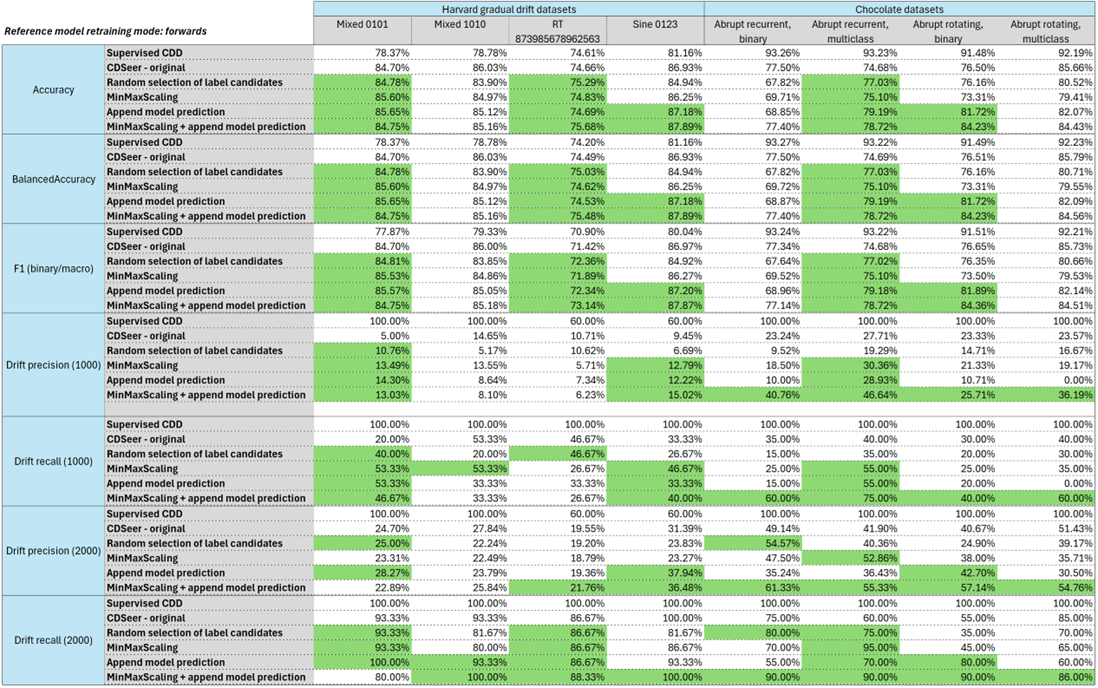
\includegraphics[scale=.95]{figures/Fig28_SVC_2.png}
 	\caption{Results for Harvard and Chocolate datasets with SVC reference model, in forwards retraining mode}
 	\label{fig:fig28}
 \end{figure}
 
 
 %\subsection{CHOCOLATE}
 
 \begin{figure}
 	\centering
 	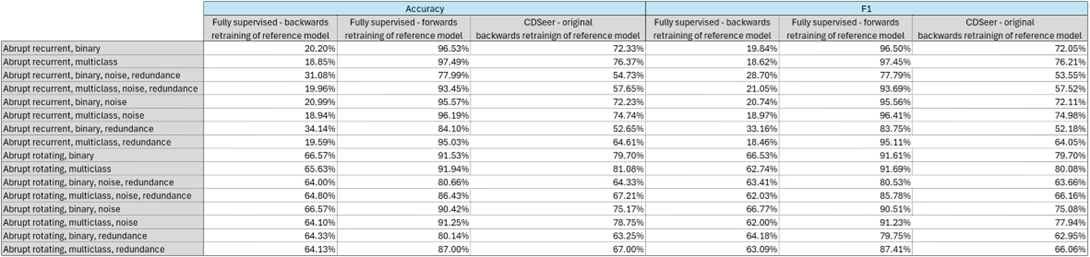
\includegraphics[scale=.95]{figures/Fig29_Chocolate_1.png}
 	\caption{Results for Chocolate datasets - BalancedAccuracy and F1}
 	\label{fig:fig29}
 \end{figure}
 
 \begin{figure}
 	\centering
 	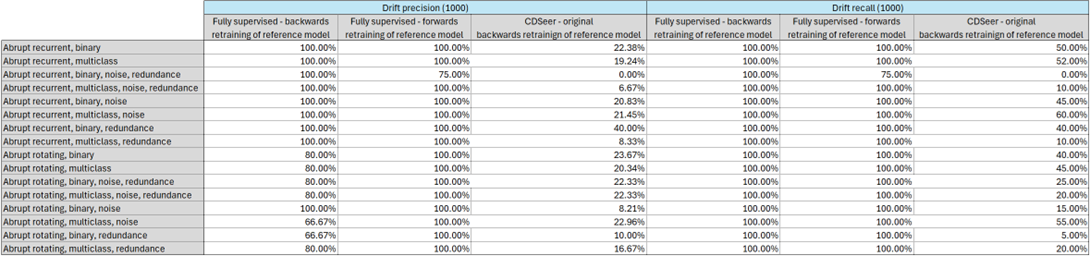
\includegraphics[scale=.95]{figures/Fig30_Chocolate_2.png}
 	\caption{Results for Chocolate datasets - Drift Precision and Recall at 1000 step tolerance}
 	\label{fig:fig30}
 \end{figure}
 
 \begin{figure}
 	\centering
 	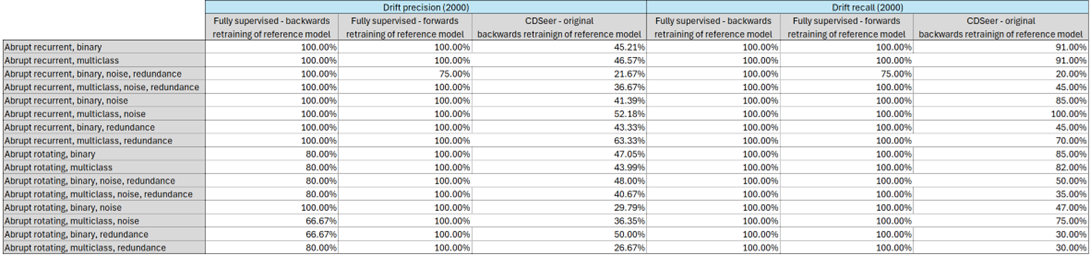
\includegraphics[scale=.95]{figures/Fig31_Chocolate_3.png}
 	\caption{Results for Chocolate datasets - Drift Precision and Recall at 2000 step tolerance}
 	\label{fig:fig31}
 \end{figure}
 
 
 %\subsection{Harvard Gradual Drift}
 \begin{figure}
 	\centering
 	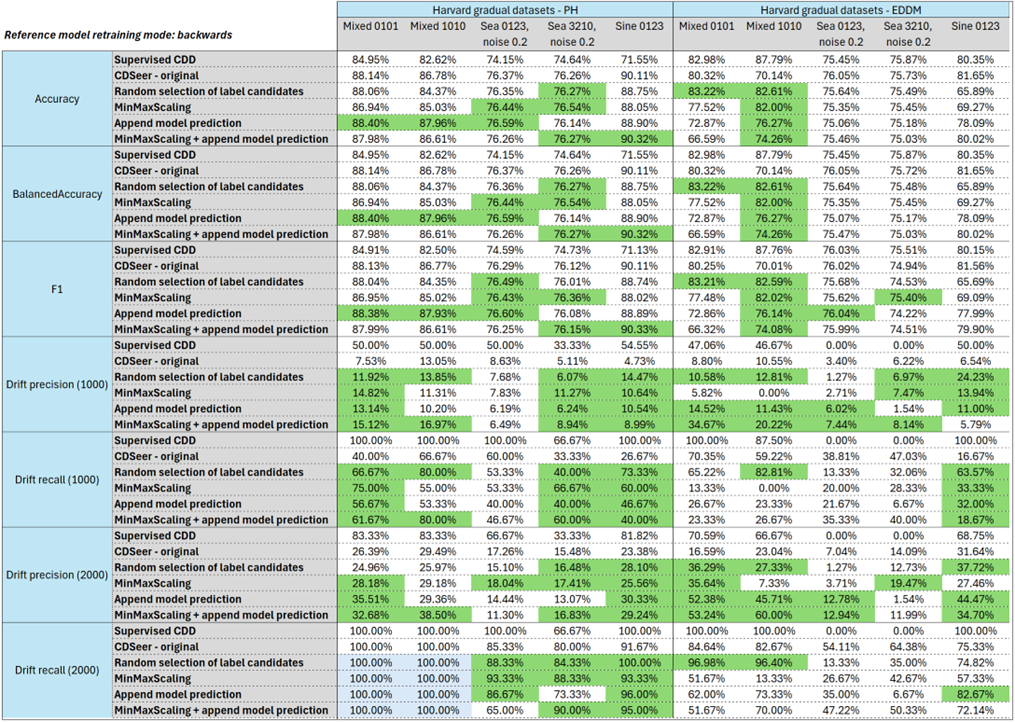
\includegraphics[scale=1]{figures/Fig32_Harv_1.png}
 	\caption{Results for Harvard datasets with PageHinkley and EDDM detectors, in backwards retraining mode}
 	\label{fig:fig32}
 \end{figure}
 
 
 \begin{figure}
 	\centering
 	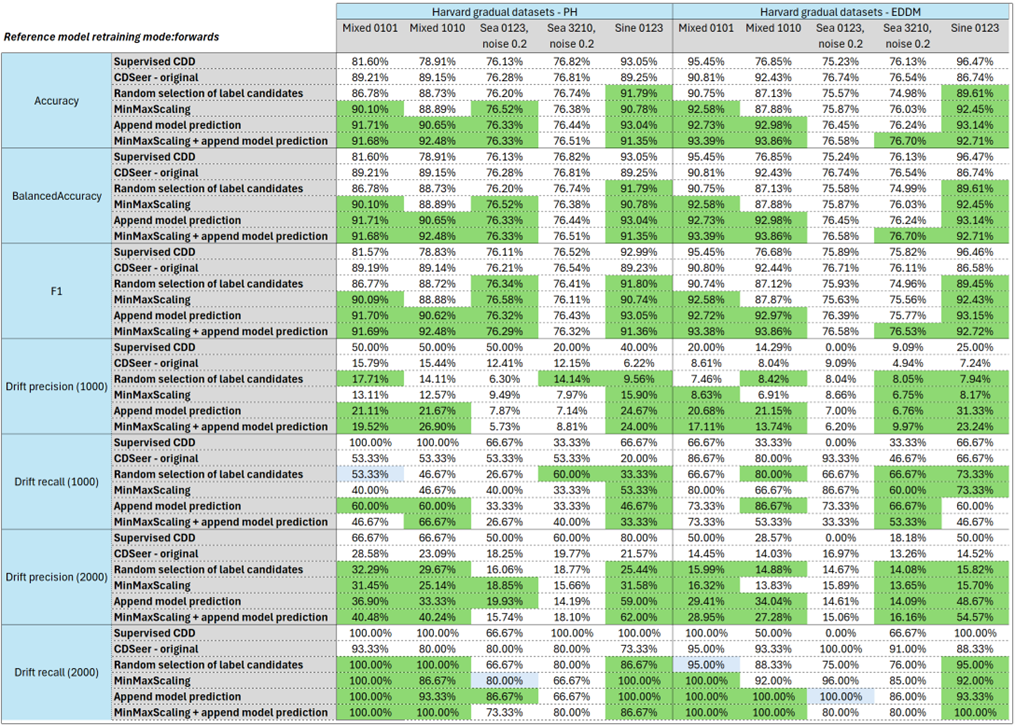
\includegraphics[scale=1]{figures/Fig33_Harv_2.png}
 	\caption{Results for Harvard dataset with PageHinkley detector, in forwards retraining mode}
 	\label{fig:fig33}
 \end{figure}
 
\end{document}


%\begin{table}
%	\caption{This is a table}
%	\begin{center}
%		\begin{tabular}{rlc}
%			\hline
%			\multicolumn{1}{l}{Year}&\multicolumn{1}{l}{World}&\multicolumn{1}{l}{Duration}\\
%			\hline
%			8000 B.C.  &     5,000,000 &  10\\
%			50 A.D.  &   200,000,000 &  20\\
%			1650 A.D.  &   500,000,000 &  30\\
%			\hline
%		\end{tabular}
%	\end{center}
%\end{table}